\section{Appendix to Section \ref{sect:sound:proofSystem} -- Soundness of the Hoare Logics}

\subsection{Expectations}
\begin{axiom}
\label{lemma:axiom:enc:assert:ul}
\label{ax:ul:sound}
We require a sound logic of assertions ($M \vdash A$), and a sound Hoare logic , \ie that for all $M$, $A$, $A'$, $stmt$:
\begin{center}
$M \vdash A   \ \ \ \  \Longrightarrow  \ \ \ \  \forall \sigma.[\ M, \sigma \models A\ ]$.\\
% \end{center}
%\end{axiom}
%
%\noindent
%Moreover, we assume that the  \ie for all $A$, $A'$, $stmt$:\ \ \  
%
%\begin{axiom}
% \begin{center}
{$M\ \vdash_{ul}\  \triple A {stmt} {A'}  \ \ \ \  \Longrightarrow  \ \ \ \ \satisfies  {M} { \triple A {stmt} {A'}}$ }
 \end{center}
\end{axiom}

\subsection{\Scoped satisfaction of assertions}
\label{s:scoped:mean}

\begin{definition}% [State Restriction, and Multi-level Sartisfaction]
\label{def:restrict}
For a state $\sigma$, and a number $i\in \mathbb{N}$ with $i \leq \DepthSt {\sigma}$,   module $M$, and assertions $A$, $A'$ we define: % $\RestictTo {\sigma} {i}$:
\begin{itemize}
\item
$  \satDAssertFrom M  \sigma k   A  \ \  \ \triangleq \  \ \  
  k\leq  \DepthSt {\sigma} \ \wedge \  \forall i\!\in\![k...\DepthSt {\sigma}].[\ M,{\RestictTo {\sigma}{i}} \models A[\overline{ {{\interpret \sigma z}/ z}}]\ ] \ \  \mbox{where} \ \
  \overline z=\fv(A).$ 
\end{itemize}
\end{definition}
 
 Remember the definition of  $\RestictTo  \sigma k$, which returns a new state whose top frame is the $k$-th frame from $\sigma$. Namely, $\RestictTo {(\phi_1...\phi_i...\phi_n,\chi)} {i}\ \ \ \triangleq \ \ \ (\phi_1...\phi_i,\chi)$
  
 
\begin{lemma}
\label{l:shallow:scoped}
For a states $\sigma$, $\sigma'$, numbers $k,k'\in \mathbb{N}$, assertions  $A$, $A'$, frame $\phi$ and variables $\overline z$, $\overline u$:
\begin{enumerate}
\item
$ \satDAssertFrom M  \sigma { \DepthSt \sigma}   A \ \ \Longleftrightarrow\ \ M,\sigma \models A\ $
\item
$ \satDAssertFrom M  \sigma {k} A \ \wedge\  k\leq k'\  \  \   \Longrightarrow \ \ \satDAssertFrom M  \sigma {k'} A$ 
\item 
\label{shallow:to:scoped}
$ M,\sigma \models A \ \wedge\ \Stable A \  \ \Longrightarrow \  \  \forall k  \leq  \DepthSt \sigma.[ \ \satDAssertFrom M  \sigma k   A \ ]$
\item
\label{fourSD}
$ M  \models A \rightarrow A'\  \  \   \Longrightarrow \ \ \forall \sigma. \forall k\leq  { \DepthSt \sigma}.[ \ \satDAssertFrom M  \sigma {k} A
\ \Longrightarrow \  \satDAssertFrom M  \sigma {k} A'\ ]$

\end{enumerate}
\end{lemma}
 
 


  
\noindent
\vspace{.1cm}
{\textbf{Proof Sketch}} 

\begin{enumerate}
\item
By unfolding and folding the definitions.
\item
By unfolding and folding the definitions.
\item
By induction on the definition of $\Stable {\_}$.
\item
  By contradiction: Assume that there exists a $\sigma$,  and a  $k\leq \DepthSt \sigma$,    such that  \\
$\strut \hspace{2cm}   \satDAssertFrom M  \sigma {k} A$ \ \ \ and \ \ \ $\neg (\satDAssertFrom M  \sigma {k} A')$\\
 The  above implies that \\
$\strut \hspace{2cm} \forall i\geq k.[\ \ M,{\RestictTo {\sigma}{i}} \models A[\overline{ {{\interpret \sigma z}/ z}}]\ \ ]$, \ \ \ and\\
$\strut \hspace{2cm} \exists j\geq k.[\ \  M,{\RestictTo {\sigma}{j}} \not\models A'[ \overline{ {{\interpret \sigma z}/ z}}]\ \ ]$,\\
 where  $\overline z \triangleq \fv(A)\cup \fv(A')$.\\
 Take $\sigma''\triangleq  \RestictTo {\sigma}{j}$. Then we have that\\
$\strut \hspace{2cm} M, \sigma'' \models A[\overline{ {{\interpret \sigma z}/ z}}]$,  and  $M,  \sigma'' \not\models A'[\overline{ {{\interpret \sigma z}/ z}}]$.\\
 This contradicts $ M  \models A \rightarrow A'$.\\
% SD I chopped the below, because I increase the set $\overline z$.
% Note that here we are also using the property that $M \models A$  and $u\notin \fv(A)$ implies $M \models A[z/u]$ -- this is needed because we have free variables in $A$ which are not free in $A[...]$ 
 {\footnoteSD{NOTE TO AUTHORS  proof hinges on the fact that we consider the "restricted" state, $\sigma''$ a "dully-fledged" state, and the fact that we no longer require "Arising".}}
 {\footnoteSD{SD  wondered whether  \ref{l:shallow:scoped}.\ref{four} would still hold if we allowed the assertions to "reflect" on the frame, to say things eg like "this and x are the only local variables". But such assertions would not have the property \ref{l:shallow:scoped}.\ref{fiveSD}}}
\end{enumerate}
\noindent
%\vspace{.1cm}
{\textbf{End Proof Sketch}} 

 
 
Finally, the following lemma allows us to combine shallow and \scoped satisfaction:

\begin{lemma}
\label{l:shallow:scoped:scoped}
For states  $\sigma$,  $\sigma'$, frame $\phi$ such that $\sigma'=\sigma  \pushSymbol \phi$, and for  
assertion $A$, such that $fv(A)=\emptyset$:
\begin{itemize}
\item
$\satDAssertFrom M  \sigma k A\   \wedge \ M, \sigma' \models A \ \ \ \Longleftrightarrow \ \ \   \satDAssertFrom M  {\sigma'} k  A$ 
\end{itemize}
\end{lemma}

\begin{proof}
By structural induction on $A$, and unfolding/folding the definitions.
\end{proof}




\subsection{Shallow and \Scoped Semantics of Hoare tuples}

Another example demonstrating that assertions at the end of a method execution might not hold after the call:

\begin{example}[$Stb^+$ not always preserved by Method Return]
\label{ex:motivate:scopes}
Assume state $\sigma_a$, such that $\interpret {\sigma_a} {\prg{this}}=o_1$, $\interpret {\sigma} {\prg{this}.f}=o_2$, $\interpret {\sigma} {x}=o_3$, $\interpret {\sigma} {x.f}=o_2$,  
and $\interpret {\sigma} {x.g}=o_4$, where $o_2$ is external and all other objects are internal. 
We then have $..,\sigma_a \models  \inside {o_4}$.
Assume %that
 the continuation of $\sigma_a$   consists of a method $x.m()$. Then,
upon entry to that method, when we push the new frame, we have  state $\sigma_b$, which also satisfies $..,\sigma_b \models  \inside {o_4}$.
Assume % that
 the   body of $m$ is $\prg{this}.f.m1(\prg{this}.g); \prg{this}.f := \prg{this};  \prg{this}.g := \prg{this}$, and % that 
 the external method $m1$ stores in the 
receiver a reference to the argument.
Then, at the end of method execution, and before popping the stack, we have   state $\sigma_c$, which also satisfies $..,\sigma_c \models  \inside {o_4}$.
However, after we pop the stack, we obtain $\sigma_d$, for which $..,\sigma_d \not\models  \inside {o_4}$.
\end{example} 


\begin{definition}[\Scoped Satisfaction of Quadruples by States]
\label{def:restrict}
For modules $\Mtwo$, $M$, state $\sigma$,  
and assertions $A$, $A'$ and  $A''$
\begin{itemize}
\item
$ {\satDAssertQuadrupleFrom \Mtwo  M  \sigma   {A} {A'} {A''} } \ \ \triangleq \ \ $  \\
$\strut \hspace{.5cm} \forall k, \overline{z}, \sigma',\sigma''.[
  \satDAssertFrom M  \sigma k   {A}  \  
  \ \Longrightarrow$\\
$\strut \hspace{4.5cm}    [ \ {\leadstoBoundedStarFin {M\madd \Mtwo}{\sigma}  {\sigma'} }\  \Rightarrow \    \satDAssertFrom M  {\sigma'} k   {\sdN{A'}}   \ ]
%[\overline{\interpret \sigma z/z}]}} \ ]
 \ \wedge$\\
$\strut \hspace{4.5cm}    [ \ {\leadstoBoundedStar  {M\madd \Mtwo}{\sigma}  {\sigma''} }\  \Rightarrow\      \satDAssertFrom M  {\sigma''}  k  {(\externalexec \rightarrow A''[\sdN{\overline{\interpret \sigma z/z}}])} \ ] $\\
$\strut \hspace{2.3cm}\ \ \ \ ]  $ \\
$\strut \hspace{2.3cm}\ \ \ \  \mbox{where }  \sdN{ \overline z= \fv(A)}$ %\!\setminus\! \vs(\sigma.\prg{cont}),\ \overline w=\fv(A)  $ 
\end{itemize}
\end{definition}



 
\begin{lemma} 
For all $M$, $\Mtwo$ $A$, $A'$, $A''$ and $\sigma$:
\begin{itemize}
\item
$ {\satDAssertQuadrupleFrom \Mtwo  M  \sigma   {A} {A'} {A''} } \ \Longrightarrow \ \
  {\satAssertQuadruple  \Mtwo  M   {A}  \sigma  {A'} {A''} } $
\end{itemize}
\end{lemma}

\label{sect:HLmeans}

We  define the {\emph {meaning}} of  our Hoare triples, $\triple {A} {stmt} {A'}$,  in the usual way, \ie that execution of $stmt$ in a state that satisfies $A$ leads to a state which satisfies $A'$.  
In addition to that, Hoare quadruples, $\quadruple {A} {stmt} {A'} {A''}$, promise that any external future states scoped by $\sigma$ will satisfy $A''$.
We give both a weak and a shallow version of the semantics


 \begin{definition}[\Scoped Semantics of Hoare triples]
For modules $M$, and assertions $A$, $A'$   we define:
%  the semantics of Hoare-triples,   $M\ \models\  \{\, A \,  \}\ stmt\  \{\, A' \, \}$ as follows:
\begin{itemize}
\item
\label{def:hoare:sem:one}
$\satisfies  {M} {  \{\, A \,  \}\ stmt\  \{\, A' \, \} }\ \ \ \triangleq$\\
{$\strut  \ \ \ \forall    \Mtwo. \forall  \sigma.[ \ \   %\arising{\sigma}{M\madd \Mtwo }\   \wedge\  
 \sigma.\prg{cont}\txteq stmt\   \Longrightarrow \ 
{\satAssertQuadruple  \Mtwo  M   {\  A\ }  \sigma  { A'  } {true} } \ \ ]$%  \ \ \  ]  $
}
 \item
 \label{def:hoare:sem:two}
$\satisfies {M} {\quadruple {A} {stmt} {A'} {A''}}  \ \ \  \triangleq$ \\
{$\strut  \ \ \  \forall    \Mtwo. \forall  \sigma.[ \  \  \sigma.\prg{cont}\txteq stmt\   \Longrightarrow \ 
{\satAssertQuadruple  \Mtwo  M    {\  A\ }  \sigma  { A'  } {A''} } \ \ ]$%  \ \ \  ]  $
}
\item
\label{def:hoare:sem:three}
$\satisfiesD {M} {  \{\, A \,  \}\ stmt\  \{\, A' \, \} }\ \ \ \triangleq$\\
{$\strut  \ \ \ \forall    \Mtwo. \forall  \sigma.[ \ \   %\arising{\sigma}{M\madd \Mtwo }\   \wedge\  
 \sigma.\prg{cont}\txteq stmt\   \Longrightarrow \ 
{\satDAssertQuadrupleFrom \Mtwo  M  \sigma   {\  A\ } { A'  } {true} } \ \ ]$%  \ \ \  ]  $
}
 
 \item
 \label{def:hoare:sem:four}
$\satisfiesD {M} {\quadruple {A} {stmt} {A'} {A''}}  \ \ \  \triangleq$ \\
{$\strut  \ \ \  \forall    \Mtwo. \forall  \sigma.[ \ \    \sigma.\prg{cont}\txteq stmt\   \Longrightarrow \ 
{\satDAssertQuadrupleFrom \Mtwo  M  \sigma   {\  A\ } { A'  } {A''} } \ \ ]$%  \ \ \  ]  $
}

\end{itemize}
\end{definition}



 
 \begin{lemma}[\Scoped   vs Shallow Semantics of Quadruples]
For all $M$, $A$, $A'$, and $stmt$:
\begin{itemize}
\item
$\satisfiesD {M} {\quadruple {A} {stmt} {A'} {A''}}   \ \ \ \Longrightarrow \ \ \ \satisfies  {M} {\quadruple {A} {stmt} {A'} {A''}} $
\end{itemize}
\end{lemma}
 \begin{proof}
 By unfolding and folding the definitions
 \end{proof}
 
 
\subsection{\Scoped satisfaction of specifications} 
%\subsection{\Scoped satisfaction of specifications -- \red{better term than \Scoped?}}  
\label{sect:HLmeans}



We now give a \scoped meaning to specifications: 

\begin{definition} [\Scoped Semantics of  Specifications]

We define $\satisfiesD{M}{{S}}$ by cases: %  over the three possible syntactic forms.

\label{def:necessity-semantics:strong}

\begin{enumerate}
\item
{ 
$\satisfiesD{M}{\TwoStatesN {\overline {x:C}} {A}} \ \  \ \triangleq   \ \ \ 
\forall \sigma.[\  \satisfiesD {M} {\quadruple {\externalexec \wedge \overline {x:C} \wedge A} {\sigma} {A} {A} } \ ] $
}
  \item
 {$\satisfiesD{M} { \mprepostN {A_1}{p\ D}{m}{y}{D}{A_2} {A_3}    }\  \ \ \   \triangleq  \ \ \ $}\\ 
 {
$\strut  \ \ \   \ \ \ \ \ \ \ \ \   \    \forall   y_0,\overline y, \sigma[ \ \ \ \sigma\prg{cont}\txteq {u:=y_0.m(y_1,..y_n)} \ \ \Longrightarrow \ \ 
\satisfiesD {M} {\quadruple  {A_1'} }   {\sigma}   {A_2' } {A_3' }  \  \ \  ]$ } \\
$\strut \ \ \   \ \ \ \ \ \ \ \ \   \  \mbox{where}$\\
$\strut  \ \ \   \ \ \ \ \ \ \ \ \   \  \ A_1' \triangleq   y_0:D,{\overline {y:D}}   \wedge   A[y_0/\prg{this}],\  \  A_2' \triangleq A_2[u/res,y_0/\prg{this}],\ \ A_3' \triangleq A_3[y_0/\prg{this}] $
 \item
 $\satisfiesD{M}{S\, \wedge\, S'}$\ \ \  \ \ \  $\triangleq$  \  \ \  \   $\satisfiesD{M}{S}\ \wedge \ \satisfiesD{M}{S'}$
\end{enumerate}
\end{definition}

 \begin{lemma}[\Scoped   vs Shallow Semantics of Quadruples]
For all $M$, $S$:
\begin{itemize}
\item
$\satisfiesD {M} {S}   \ \ \ \Longrightarrow \ \ \ \satisfies  {M} {S} $
\end{itemize}
\end{lemma}

\subsection{Soundness of the Hoare Triples Logic}
\label{s:sound:app:triples}

\begin{auxLemma}
\label{l:no:call}
For any module $M$, assertions $A$, $A'$ and $A''$, such that $\Pos A$, and $\Pos {A'}$, and a statement $stmt$ which does not contain any method calls:
\begin{center}
$  \satisfiesD {M} {\triple {A} {stmt} {A'} }  \ \ \Longrightarrow\ \  \satisfiesD {M} {\quadruple {A} {stmt} {A'} {A''}}$
\end{center}
\end{auxLemma}

\begin{proof}

\end{proof}

%%%%%%%%%%%%%%%%%%%%%%%%%%%%%%%%%%%%%%%%%%%%%%%%%%%%%%%%%%%%%%%%%%%%

%%%%%%%%%%%%%%%%%%%%%%%%%%%%%%%%%%%%%%%%%%%%%%%%%%%%%%%%%%%%%%%%%%%%
\subsubsection{Lemmas about protection}
\label{s:app:protect:lemmas}

\begin{definition}

$\LRelevantKO  {\sigma} {k}\ \ \ \triangleq\ \ \  \{ \alpha \mid  \exists i.[ \ k \leq i \leq \depth \sigma \ \wedge \ \alpha \in \LRelevantO  {\RestictTo \sigma i}\ ]$
\end{definition}
 
Lemma \ref{exec:rel} guarantees that  program execution reduces the locally reachable objects, unless it allocates new ones.
That is, any objects locally reachable in the $k$-th frame of the new state ($\sigma'$), are either new, or were locally reachable in the $k$-th frame of the previous state ($\sigma$).

{
\begin{lemma} For all $\sigma$, $\sigma'$, and $\alpha$, where $\models \sigma$, and where $k\leq \DepthSt {\sigma}$:
\label{exec:rel}
\begin{itemize}
\item
$\leadstoBounded  {\Mtwo\cdot M}  {\sigma}  {\sigma'}\ \  \Longrightarrow\ \ 
  \LRelevantKO   {\sigma'} {k}\cap \sigma   \subseteq\   \LRelevantKO {\sigma} {k}  $
\item
$\leadstoBoundedStar  {\Mtwo\cdot M}  {\sigma}  {\sigma'}\ \  \Longrightarrow\ \ 
  \LRelevantKO   {\sigma'} {k}\cap \sigma   \subseteq\   \LRelevantKO {\sigma} {k} $
\end{itemize}
\end{lemma}
 }
 
\begin{proof} $~ $

\begin{itemize}
\item
If the step is a method call, then the assertion follows by construction.
If the steps is a   local execution in a method, we proceed by case analysis. If it is an assignment to a local variable, then 
$\forall k.[\ \LRelevantKO   {\sigma'} {k}= \LRelevantKO   {\sigma} {k}\ ]$.
If the step is the creation of a new object, then the assertion holds by construction.
If it it is a field assignment, say, $\sigma'=\sigma[\alpha_1,f \mapsto \alpha_2]$, then we have that 
$\alpha_1, \alpha_2 \  \LRelevantKO {\sigma} {\DepthSt \sigma}$. 
And therefore, by Lemma \ref{rel:smaller}, we also have that $\alpha_1, \alpha_2 \  \LRelevantKO {\sigma} {k}$
All locally reachable objects in $\sigma'$ were either already reachable in $\sigma$ or reachable through $\alpha_2$,
Therefore, we also have that  $\LRelevantKO   {\sigma'} {k}\subseteq  \LRelevantKO   {\sigma} {k}$
 And by definition of $\leadstoBounded  {\_}  {\_}  {\_}$, it is not a method return.
 
\item
By induction on the number of steps in $\leadstoBoundedStar  {\Mtwo\cdot M}  {\sigma}  {\sigma'}$. 
For the steps that correspond to method calls, the assertion follows by construction.
For the steps that correspond to local execution in a method, the assertion follows from the bullet above.
For the steps that correspond to method returns, the assertion follows by lemma \ref{rel:smaller}.
\end{itemize}
\end{proof}

Lemma \ref{change:external} guarantees that any change to the contents of an external object can only happen during execution of an external method.
 
 {
 \begin{lemma} For all $\sigma$, $\sigma'$:
 \label{change:external}
\begin{itemize}
\item
$\leadstoBounded  {\Mtwo\cdot M}  {\sigma}  {\sigma'}\ \wedge \  \sigma \models \external{\alpha} \ \wedge\  {\interpret{\sigma} {\alpha.f}} \neq {\interpret{\sigma'} {\alpha.f}}
 \ \ \Longrightarrow\ \  M,\sigma \models \extThis$
\end{itemize}
\end{lemma}
  } 
  \begin{proof}
  Through inspection of the operational semantics in Fig. \ref{f:loo-semantics}, and in particular rule {\sc{Write}}.
  \end{proof}  
  
 
%   {
% \begin{lemma} For all $\sigma$, $\sigma'$, and $\alpha$:
% \label{lemma:notInside:implies}
%\begin{itemize}
%\item
%$ \satDAssertFrom M  {\sigma} k   {\inside{\alpha}}  \ \wedge \ \leadstoBounded  {\Mtwo\cdot M}  {\sigma}  {\sigma'}\ \wedge \  \notSatDAssertFrom M  {\sigma'} k   {\inside{\alpha}}
% \ \ \Longrightarrow\ \ $\\
% $\exists \alpha_o,f.[\  \alpha_0 \in \LRelevantKO  {\sigma} {k} \ \wedge \ M, \sigma' \models \external {\alpha_o} \ \wedge \ \interpret {\sigma'} {\alpha_o.f} = \alpha\  \wedge$\\
%$\strut \hspace{3cm} [ \alpha_o \notin \sigma\ \vee\ \alpha_o \notin \LRelevantKO {\sigma} {k}\ \vee\  \interpret {\sigma} {\alpha_o.f} \neq \alpha\ ]\ \ \ \ \ ] $
%\end{itemize}
%\end{lemma}
%}

Lemma \ref{lemma:inside:preserved}  guarantees that internal code which does not include method calls preserves absolute protection. 
It is used in the proof of soundness of the inference rule {\sc{Prot-1}}.

  {
 \begin{lemma} For all $\sigma$, $\sigma'$, and $\alpha$:
 \label{lemma:inside:preserved} 
\begin{itemize}
\item
$ \satDAssertFrom M  {\sigma} k   {\inside{\alpha}}  \, \wedge \,M, \sigma \models \intThis \, \wedge \, \sigma.\prg{cont} \mbox{ contains no method calls } \ \wedge\ \leadstoBounded   {\Mtwo\cdot M}  {\sigma}  {\sigma'}\  \ \ \Longrightarrow\ \ \satDAssertFrom M  {\sigma'} k   {\inside{\alpha}}$
\item
$ \satDAssertFrom M  {\sigma} k   {\inside{\alpha}}  \ \wedge \ M, \sigma \models \intThis \ \wedge \ \sigma.\prg{cont}  \mbox{ contains no method calls } \ \wedge\ \leadstoBoundedStar  {\Mtwo\cdot M}  {\sigma}  {\sigma'}\  \ \ \Longrightarrow\ \ \satDAssertFrom M  {\sigma'} k   {\inside{\alpha}}$
\end{itemize}
\end{lemma}
}

\begin{proof} $~ $

\begin{itemize}
\item
Because $\sigma.\prg{cont}$   contains no method calls, we also have that $\DepthSt {\sigma'}=\DepthSt {\sigma}$. Let us take
$m=\DepthSt {\sigma}$.

We continue by contradiction.
 Assume that $\satDAssertFrom M  {\sigma} k   {\inside{\alpha}}$ and $\notSatDAssertFrom M  {\sigma} k   {\inside{\alpha}}$  

Then:\\
(*)\ $\forall f.\forall i\in [k..m].\forall \alpha_o\in  \LRelevantKO {\sigma} {i}.[\ M, \sigma \models \external {\alpha_o} \Rightarrow \interpret {\sigma} {\alpha_o.f} \neq \alpha\ \wedge \alpha_o \neq \alpha \ ] $.
\\
(**) $\exists f.\exists  j\in [k..m].\exists \alpha_o\in  \LRelevantKO {\sigma'} {j}.[\ M, \sigma' \models \external {\alpha_o} \wedge \interpret {\sigma'} {\alpha_o.f} = \alpha\ \vee \alpha_o = \alpha\ ] $
\\
We proceed by cases
\begin{description}
\item{1st Case} $\alpha_o \notin  \sigma$, \ie $\alpha_o$ is a new object.
  Then, by our operational semantics, it cannot have a field pointing to an already existing object ($\alpha$), nor can it be equal with $\alpha$. Contradiction.
\item{2nd Case}  $\alpha_o \in  \sigma$. Then, by Lemma \ref{exec:rel}, we obtain that $\alpha_o \in \LRelevantKO {\sigma} {j}$.
Therefore, using (*), we obtain that $\interpret {\sigma} {\alpha_o.f} \neq \alpha$, and therefore 
$ \interpret {\sigma} {\alpha_o.f} \neq \interpret {\sigma'} {\alpha_o.f}$.
By lemma \ref{change:external}, we obtain $M, \sigma \models \extThis$. Contradiction!
\end{description}

\item
By induction on the   number of steps, and using the bullet above.
\end{itemize}

\end{proof}

% \subsubsection{Lemmas about relative protection}

 
  {
 \begin{lemma} For all $\sigma$, $\sigma'$, and $\alpha$:
 \label{lemma:protTwo}
\begin{itemize}
\item
$  M, \sigma  \models    { \protectedFrom \alpha {\alpha_o}}  \ \wedge\   \sigma.\prg{heap}= \sigma'.\prg{heap} \ \ \Longrightarrow\ \  M, \sigma' \models      { \protectedFrom \alpha {\alpha_o}} $
\end{itemize}
\end{lemma}
}

\begin{proof}
By unfolding and folding the definitions.
\end{proof}

{
 \begin{lemma} For all $\sigma$,  and $\alpha$, $\alpha_o$, $\alpha_1$, $\alpha_2$:
 \label{l:prtFrom}
\begin{itemize}
\item
$ M, \sigma  \models    {\protectedFrom \alpha  {\alpha_o}}  \  \wedge \ \  M, \sigma  \models    {\protectedFrom \alpha  {\alpha_1}}    \   \ 
\Longrightarrow\ \ M, \sigma[\alpha_2,f \mapsto \alpha_1] \models  \protectedFrom\alpha   {\alpha_o}$
\end{itemize}
\end{lemma}
}

{
\begin{definition}
\begin{itemize}
\item
$M, \sigma \models \internalPaths{\re} \ \ \triangleq \ \ \forall \overline{f}.[\  M, \sigma \models \internal{\re.\overline{f}}\ ]$
\end{itemize}
\end{definition}
}

{
 \begin{lemma} For all $\sigma$, and $\alpha_o$ and $\alpha$:
\begin{itemize}
\item
$M, \sigma \models \internalPaths{\alpha_o}  \    \ \ \Longrightarrow\ \ M, \sigma \models {\protectedFrom \alpha {\alpha_o}}$
\end{itemize}
\end{lemma}
}

\noindent
\vspace{.2cm}
\textbf{Proof Sketch Theorem \ref{l:triples:sound}} 
The proof goes by case analysis over the rule applied to obtain $M \vdash \{ A \}\ stmt \  \{ A' \} $:

\begin{description} 

\item[{\sc{extend}}] 
By  soundness of the underlying Hoare logic (axiom \ref{ax:ul:sound}), we obtain that  $M\ \models\ \triple {A} {stmt}   {A'}$.
By axiom \ref{ax:ul} we also obtain that $\Stable{A}$ and  $\Stable{A'}$. 
This, together with   Lemma \ref{l:shallow:scoped}, part \ref{shallow:to:scoped}, gives us that
$\satisfiesD {M} {\triple {A} {stmt} {A'} }$. 
By the assumption of {\sc{extend}}, $stmt$ does not contain any method call. Rest follows by lemma \ref{l:no:call}.

\item[{\sc{Prot-New}}] By operational semantics, no field of another object will point to $u$, and therefore $u$ is protected, and protected from all variables $x$.

\item[{\sc{Prot-1}}] by Lemma \ref{lemma:inside:preserved}. The rule premise
${\hproves{M}  	{\ z=e   } {\ stmt } {\ z=e\  }}$ allows us to consider addresses, $\alpha$,   rather than expressions, $e$.


\item[{\sc{Prot-2}}] by Lemma \ref{lemma:protTwo}. The rule premise
${\hproves{M}  	{\ z=e \wedge z=e'\ } {\ stmt } {\ z=e \wedge z=e'\ }}$ allows us to consider addresses $\alpha$, $\alpha'$ rather than expressions $e$, $e'$.

\item[{\sc{Prot-3}}] also by Lemma \ref{lemma:protTwo}. Namely, the rule does not change, and $y.f$ in the old state has the same value as $x$ in the new state.

\item[{\sc{Prot-4}}] by Lemma \ref{l:prtFrom}.

\item[{\sc{types-1}}] 

Follows from type system, the assumption of {\sc{types-1}} and lemma \ref{l:no:call}.


\end{description}
\noindent
\vspace{.1cm}
{\textbf{End Proof Sketch}} 



\subsection{Well-founded ordering}

 \begin{definition}
\label{def:measure}
For a module $M$, and modules $\Mtwo$,   we define a measure, $\measure {A, \sigma,A',A''} {M,\Mtwo} $, and based on it, a well founded ordering $(A_1,\sigma_1,A_2, A_3) \ll_{M,\Mtwo}  (A_4,\sigma_2,A_5,A_6)$
as follows:
\begin{itemize}
\item
 $\measure {A, \sigma,A',A''} {M,\Mtwo} \  \ \triangleq \ \  (m, n)$,  \ \ \  where
\begin{itemize}
\item
$m$ is the minimal number of execution steps so that $ \leadstoBoundedStarFin {M\cdot \Mtwo} {\sigma}    {\sigma'}$  for some $\sigma'$, {and $\infty$ otherwise}.
 \item
  $n$ is minimal depth of all proofs of $M \vdash \quadruple {A} {\sigma.\prg{cont}} {A'} {A''} $.
\end{itemize}
 \item
 $(m,n) \ll (m',n')$\ \  \ \ $\triangleq$ \ \  \ \ $ m<m'\vee  (m=m'  \wedge n < n')   $.
\item
$(A_1,\sigma_1,A_2, A_3) \ll_{M,\Mtwo}  (A_4,\sigma_2,A_5, A_6)$  \  \  $\triangleq$ \ \ 
$\measure {A_1, \sigma_1,A_2, A_3} {M,\Mtwo}  \ll \measure {A_4, \sigma_2,A_5. A_6} {M,\Mtwo} $
\end{itemize}
\end{definition}

%\subsection{Our Well-founded ordering}

\begin{lemma}
\label{lemma:normal:two}
For any modules $M$ and $\Mtwo$,  the relation $\_ \ll_{M,\Mtwo}  \_$ is well-founded.
\end{lemma}

%%%%%%%%%%%%%%%%%%%%%%%%%%%%%%%%%%%%%%%%%%%%%%%%%%%%%%%%%%

\subsection{Public States, properties of executions consisting of several steps}

We t define a state to be public, if the currently executing method is public.

\begin{definition}
We use the form
$M, \sigma \models \pubMeth$ to express that the currently executing method is public.\footnote{This can be done by looking in the caller's frame -- ie the one right under the topmost frame -- the class of the current receiver and the name of the currently executing method, and then looking up the method definition in the module $M$; if not defined there, then it is not \prg{public}. }
Note that $\pubMeth$ is not part of the assertion language.
\end{definition}

 \begin{auxLemma}[Enclosed Terminating Executions]\footnoteSD{TODO find better name for the aux lemma}
 \label{lemma:encl:tem}
 For   modules $\Mtwo$,   states $\sigma$, $\sigma'$, $\sigma_1$:
\begin{itemize}
\item
$  \leadstoBoundedStarFin {\Mtwo}  {\sigma}  {\sigma'} \  \wedge \  \leadstoBoundedStar  {\Mtwo}  {\sigma}  {\sigma_1} 
% $\\ $
\ \ \  \Longrightarrow\ \ \  % $\\ $  
 \exists \sigma_2.[\ \ \leadstoBoundedStarFin {\Mtwo} {\sigma_1}  {\sigma_2}  
\ \wedge\ 
\leadstoBoundedStarThree  {\Mtwo}  {\sigma_2}  {\sigma}   {\sigma'} \ \ ]$
\end{itemize}

\end{auxLemma} 

\begin{auxLemma}[Executing  sequences]
\label{lemma:subexp}
For modules $\Mtwo$, statements $s_1$, $s_2$,  states $\sigma$, $\sigma'$, $\sigma'''$:
\begin{itemize}
\item
$ \sigma.\texttt{cont} = s_1; s_2 \ \ \wedge\ \  \leadstoBoundedStarFin {\Mtwo}  {\sigma}  {\sigma'}\ \ 
\wedge \ \
\leadstoBoundedStar {\Mtwo}  {\sigma}  {\sigma''}\
$\\
$  \Longrightarrow$\\
$   \exists \sigma''.[\ \ \ \ \   \leadstoBoundedStarFin {\Mtwo} {\sigma[\texttt{cont}\mapsto s_1]}  {\sigma''}  
\ \wedge\ 
\leadstoBoundedStarFin {\Mtwo} {\sigma''[\texttt{cont}\mapsto s_2]}   {\sigma'} \  \wedge$
\\
$\strut \hspace{1.2cm}  [ \ \ \leadstoBoundedStar {\Mtwo} {\sigma[\texttt{cont}\mapsto s_1]}   {\sigma''}\ \vee \ \leadstoBoundedStarFin {\Mtwo}  {\sigma''[\texttt{cont}\mapsto s_2]}   {\sigma'''}\ ]\ \ \ \ \ \ \ \  \ ] $
\end{itemize}
\end{auxLemma}

\subsection{Summarised Executions}

We repeat the two diagrams given in \S \ref{s:summaized}.

\begin{tabular}{lll}
\begin{minipage}{.45\textwidth}
The diagram opposite  shows such an execution:
  $ \leadstoBoundedStarFin {\Mtwo\cdot M}    {\sigma_2}  {\sigma_{30}}$ consists of 4 calls to external objects,
and 3 calls to internal objects.
The calls to external objects are from $\sigma_2$ to $\sigma_3$,  from $\sigma_3$ to $\sigma_4$, from $\sigma_9$ to $\sigma_{10}$, 
and  from $\sigma_{16}$ to $\sigma_{17}$.
 The calls to internal objects are from $\sigma_5$ to $\sigma_6$, rom $\sigma_7$ to $\sigma_8$, and from $\sigma_{21}$ to $\sigma_{23}$. 
\end{minipage}
& \ \  &
\begin{minipage}{.4\textwidth}
\resizebox{6.2cm}{!}
{
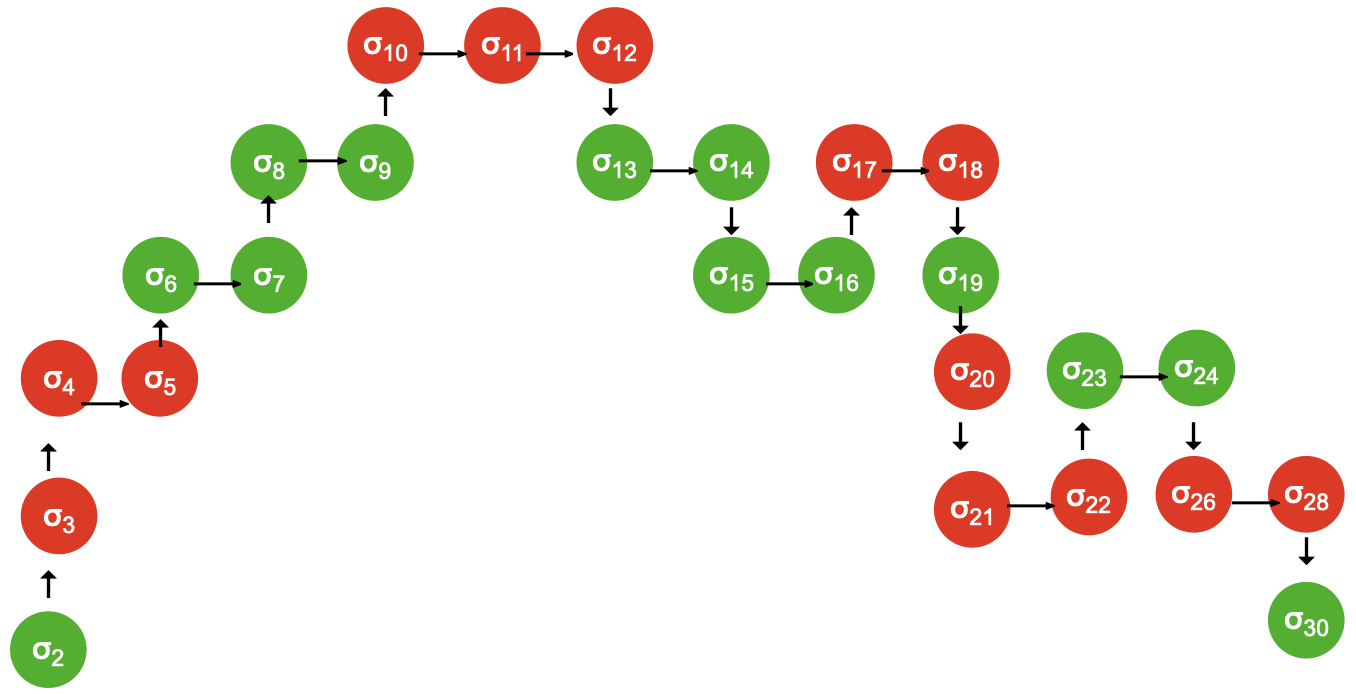
\includegraphics[width=\linewidth]{diagrams/summaryA.png}
} \end{minipage}
\end{tabular}

\begin{tabular}{lll}
\begin{minipage}{.45\textwidth}
 In terms of our example, we want to summarise the execution of the two ``outer'' internal, public methods into the 
 ``large'' steps $\sigma_6$ to $\sigma_{19}$ and $\sigma_{23}$ to $\sigma_{24}$.
 And are not concerned with the states reached from these two public method executions.  
\end{minipage}
& \ \  &
\begin{minipage}{.4\textwidth}
\resizebox{6.2cm}{!}
{
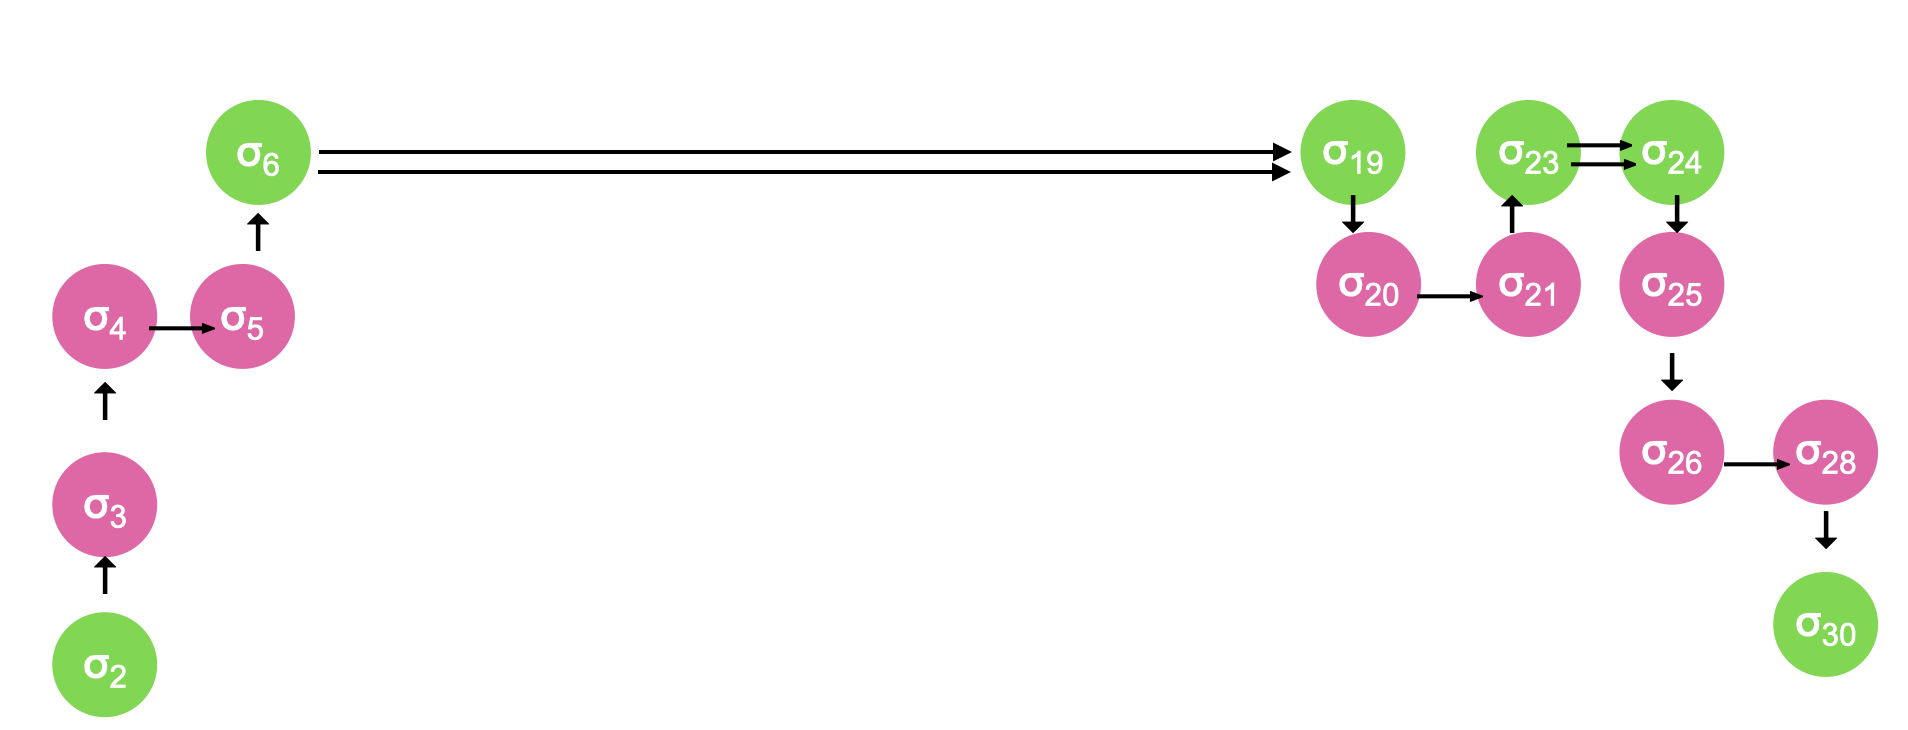
\includegraphics[width=\linewidth]{diagrams/summaryB.png}
} \end{minipage}
\end{tabular} 

\noindent 
In order to express such summaries, Def. \ref{def:exec:sum} introduces the following concepts:
\begin{itemize}
\item
 ${\leadstoBoundedThreeStarExt {\Mtwo\cdot M} {\sigma\bd}  {\sigma}  {\sigma'}}$ \ \ \  execution from $\sigma$ to $\sigma'$ scoped by $\sigma\bd$, involving  external states only.
\item
${\WithPub {\Mtwo\cdot M}    {\sigma}  {\sigma'} {\sigma_1}}$ \  \ \  \ \ \ \ \ \ \ \  ${\sigma}$ is an external state  calling an internal public method, and \\
$\strut \hspace{3.25cm}$ $\sigma'$ is the state after return from the public method, and \\
$\strut \hspace{3.25cm}$  $\sigma_1$ is the first state upon entry to the public method.  
%$\WithExtPub {\Mtwo\cdot M} {\sigma\bd}  {\sigma}  {\sigma'} {\epsilon}$ \ \     \ \  $\triangleq$ \ \ 
%$\leadstoBoundedThreeStarExt {\Mtwo\cdot M} {\sigma\bd}  {\sigma}  {\sigma''}$
%\item
%$\WithExtPub {\Mtwo\cdot M} {\sigma\bd}  {\sigma}  {\sigma'} {\sigma_1...\sigma_n}$   \ \  int
%\item
%$\leadstoBoundedExtPub {\Mtwo\cdot M}    {\sigma}  {\sigma'} $   \ \ \ \ \   \ \ \  \ \ \ \   \ \ \ \  $\triangleq$   \ \ 
%  $ \exists n\in \mathbb{N}. \exists \sigma_1,...\sigma_n. \ \WithExtPub {\Mtwo\cdot M} {\sigma}  {\sigma}  {\sigma'} {\sigma_1...\sigma_n} 
%$
\end{itemize}
  
  \noindent
Continuing with our example, we have the following execution summaries:
\begin{enumerate}
\item
${\leadstoBoundedThreeStarExt {\Mtwo\cdot M} {\sigma_3}  {\sigma_3}  {\sigma_5}}$\ \ \ 
Purely external execution from $\sigma_3$ to $\sigma_5$, scoped by $\sigma_3$.
\item
${\WithPub {\Mtwo\cdot M}    {\sigma_5}  {\sigma_{20}} {\sigma_{6}}}$. \ \ \ 
Public method call from external state $\sigma_5$ into  nternal state $\sigma_6$ returning to $\sigma_{20}$. 
Note that this   summarises two  internal method executions ($\sigma_{6}-\sigma_{19}$, and $\sigma_8-\sigma_{14}$),
and two external method executions ($\sigma_{6}-\sigma_{19}$, and $\sigma_8-\sigma_{14}$).
\item
 ${\leadstoBoundedThreeStarExt {\Mtwo\cdot M} {\sigma_3}  {\sigma_{20}}  {\sigma_{21}}}$.
 \item
${\WithPub {\Mtwo\cdot M}    {\sigma_{21}}  {\sigma_{25}} {\sigma_{23}}}$. \ \ \ 
Public method call from  external state ${\sigma_{21}}$ into internal state $\sigma_{23}$, and returning to external state $\sigma_{25}$.
 \item
  ${\leadstoBoundedThreeStarExt {\Mtwo\cdot M} {\sigma_3}  {\sigma_{25}}  {\sigma_{28}}}$.
\ \ \ 
  Purely external execution from $\sigma_{25}$ to $\sigma_{28}$, scoped by ${\sigma_3}$.
\end{enumerate}


\begin{definition}
\label{def:exec:sum}
For any module $M$  where $M$ is the internal module, external modules $\Mtwo$, and states $\sigma\bd$,  $\sigma$,  $\sigma_1$, ... $\sigma_n$, and $\sigma'$, we define:

\begin{enumerate}

% 1
\item
 ${\leadstoBoundedThreeStarExt {\Mtwo\cdot M} {\sigma\bd}  {\sigma}  {\sigma'}}$ \ \ \ \ \   $\triangleq$ \ \ 
$
\begin{cases}
M, \sigma  \models  \extThis\  \wedge\  \\
[ \ \ \ 
\sigma=\sigma' \, \wedge\,  \EarlierS  {\sigma\bd}  {\sigma} \, \wedge\,  \EarlierS  {\sigma\bd}  {\sigma''}\ \ \ \ \ \vee\\
\ \ \ \exists \sigma''[\,  \leadstoBoundedThree {\Mtwo\cdot M} {\sigma}  {\sigma\bd}   {\sigma''} \  \wedge\  
{\leadstoBoundedThreeStarExt {\Mtwo\cdot M} {\sigma\bd}  {\sigma''}  {\sigma'}}\, ] \ \ \ ]
\end{cases}
$

% 2
\item
${\WithPub {\Mtwo\cdot M}    {\sigma}  {\sigma'} {\sigma_1}}$ \  \ \  \ \ \ \ \ \ \ \ $\triangleq$ \ \ 
$\begin{cases}
M, \sigma  \models \extThis \ \wedge \\
\exists   \sigma_1'\ [ \ \   \leadstoBoundedThree  {\Mtwo\cdot M} {\sigma} {\sigma}  {\sigma_{1}}\, \wedge\,  M, \sigma_1 \models \pubMeth \ \wedge \\ 
\strut \ \ \ \ \  \ \ \ \ \ \   \leadstoBoundedStarFin {\Mtwo\cdot M} {\sigma_1}  {\sigma_1'}  \ \wedge \   \leadstoBounded  {\Mtwo\cdot M} {\sigma_1'}      {\sigma'} \ \ ] 
\end{cases}
$

% 3
\item
$\WithExtPub {\Mtwo\cdot M} {\sigma\bd}  {\sigma}  {\sigma'} {\epsilon}$ \ \      \  $\triangleq$ \ \ 
$\leadstoBoundedThreeStarExt {\Mtwo\cdot M} {\sigma\bd}  {\sigma}  {\sigma''}$

% 4 
\item
\label{four:defg23a}
$\WithExtPub {\Mtwo\cdot M} {\sigma\bd}  {\sigma}  {\sigma'} {\sigma_1}$  \ \ \  $\triangleq$ \ \ 
$\exists \sigma_1',\sigma_2'.  
\begin{cases}
 \ \   {\leadstoBoundedThreeStarExt {\Mtwo\cdot M} {\sigma\bd}  {\sigma}  {\sigma_1'}}\ \wedge\ 
{\WithPub {\Mtwo\cdot M}    {\sigma_1'}  {\sigma_2'} {\sigma_1}}  \ \ \wedge \\
 \ \  {\leadstoBoundedThreeStarExt {\Mtwo\cdot M} {\sigma\bd}  {\sigma_2'}  {\sigma'}}   \\
  \end{cases}$

 
 %5
\item
\label{four:defg23}
$\WithExtPub {\Mtwo\cdot M} {\sigma\bd}  {\sigma}  {\sigma'} {\sigma_1...\sigma_n}$   \ \  $\triangleq$ \ \ 
$\exists \sigma_1'.[ \  \
 \WithExtPub {\Mtwo\cdot M} {\sigma\bd}  {\sigma}  {\sigma_1'} {\sigma_1} 
  \ \wedge \ 
    {\WithExtPub {\Mtwo\cdot M} {\sigma\bd}  {\sigma_1'}  {\sigma'} {\sigma_2...\sigma_n} }   \  \ ]
$

% 6
\item
\label{six:g23}
$\leadstoBoundedExtPub {\Mtwo\cdot M}    {\sigma}  {\sigma'} $    \ \ \   \ \ \  \ \ \ \   \ \ \ \  $\triangleq$   \ \ 
 $ \exists n\!\in\! \mathbb{N}. \exists \sigma_1,...\sigma_n. \ \WithExtPub {\Mtwo\cdot M} {\sigma}  {\sigma}  {\sigma'} {\sigma_1...\sigma_n} 
$
\end{enumerate}
\end{definition}

\vspace{.1cm}

Note   that 
${\leadstoBoundedThreeStarExt {\Mtwo\cdot M} {\sigma\bd}  {\sigma}  {\sigma'}}$ implies that $\sigma$ is external, but does not
imply that $\sigma'$ is external.
${\leadstoBoundedThreeStarExt {\Mtwo\cdot M} {\sigma}  {\sigma}  {\sigma'}}$. 
On the other hand, $\WithExtPub {\Mtwo\cdot M} {\sigma\bd}  {\sigma}  {\sigma'} {\sigma_1...\sigma_n}$ implies that $\sigma$ and $\sigma'$ are external, and  $\sigma_1$, ... $\sigma_1$  are internal and public.
Finally, note that   in part (\ref{six:g23}) above it is possible that $n=0$, and so 
$\leadstoBoundedExtPub {\Mtwo\cdot M}    {\sigma}  {\sigma'} $  also holds when
Finally, note that the decomposition used in (\ref{four:defg23}) is not unique, but since we only care for the public states this is of no importance.

\vspace{.2cm}

Lemma \ref{lemma:external_breakdown:term} says that\\
\begin{enumerate}
\item
Any terminating execution which starts at an external state ($\sigma$) consists of a number of external states interleaved with another number of terminating calls to public methods.
\item
Any execution execution which starts at an external state ($\sigma$) and reaches another state ($\sigma'$) also consists of a number of external states interleaved with another number of terminating calls to public methods, which may be followed by a call to some public method (at $\sigma_2$), and from where another execution, scoped by $\sigma_2$  reaches $\sigma'$.
\end{enumerate}


 \begin{auxLemma}
\label{lemma:external_breakdown:term}[Summarised Executions]
For   module $M$, modules $\Mtwo$, and states $\sigma$, $\sigma'$:
\\
\\
If $M,\sigma \models \extThis$, then
\begin{enumerate}
\item
\label{lemma:external_breakdown:term:one}
$\leadstoBoundedStarFin {M\cdot \Mtwo}  {\sigma}  {\sigma'}  \ \ \  \ 
\Longrightarrow \ \ \  \ \leadstoBoundedExtPub {\Mtwo\cdot M}    {\sigma}  {\sigma'}$
\item
\label{lemma:external_breakdown:two}
$\leadstoBoundedStar  {M\cdot \Mtwo}  {\sigma}  {\sigma'}  \ \ \  \ \ \  
\Longrightarrow$ 

\begin{enumerate}
\item
$\strut \ \ \ \ \ \ \ \    \leadstoBoundedExtPub {\Mtwo\cdot M}    {\sigma}  {\sigma'}\ \ \ \  \vee$
\item
$\strut \ \ \ \ \ \ \ \    \exists \sigma_c,\sigma_d.[\ 
\leadstoBoundedExtPub {\Mtwo\cdot M}    {\sigma}  {\sigma_c} 
\wedge\ \leadstoBounded  {\Mtwo\cdot M}    {\sigma_c}  {\sigma_d} 
\wedge \ M, \sigma_c \models \pubMeth \wedge \leadstoBoundedStar  {\Mtwo\cdot M}    {\sigma_d}  {\sigma'} \ ]
$
\end{enumerate}
\end{enumerate}
\end{auxLemma}
 



\begin{auxLemma}
\label{lemma:external_exec_preserves_more}[Preservation of Encapsulated Assertions]
For any module $M$, modules $\Mtwo$,  assertion  $A$, and 
% variables $\overline x$, and addresses $\overline \alpha$,
 states $\sigma\bd$, $\sigma$, $\sigma_1$ ... $\sigma_n$, $\sigma_a$, $\sigma_b$ and $\sigma'$:

\noindent
If

\noindent
 $\strut \hspace{.5cm} M \vdash \encaps A \   \wedge   \ fv(A)=\emptyset \  \wedge \ 
\satDAssertFrom M {\sigma} k A \ \wedge \ k \leq \DepthSt {\sigma\bd}$. 

\noindent
Then

\begin{enumerate}
% ΟΝΕ
\item
\label{lemma:external_exec_preserves_more:one}
$  M, \sigma  \models \extThis \ \wedge \  \leadstoBoundedThree  {\Mtwo\cdot M} {\sigma} {\sigma\bd}  {\sigma'} 
\ \ \Longrightarrow \ \ \ \satDAssertFrom M {\sigma'} k A$

% TWO
\item
$   \leadstoBoundedThreeStarExt {\Mtwo\cdot M} {\sigma\bd}  {\sigma}  {\sigma'} 
\ \ \Longrightarrow \ \ \ \satDAssertFrom M {\sigma'} k A$

% THREE
\item
\label{lemma:external_exec_preserves_more:three}
$ \WithExtPub {\Mtwo\cdot M} {\sigma\bd}  {\sigma}  {\sigma'} {\sigma_1...\sigma_n}\ \ \wedge $\\
 $\strut \ \ \ \  \  \forall i\in [1..n]. \forall \sigma_{f}.[ \ \  \satDAssertFrom M {\sigma_i} k A  \ \wedge \  \leadstoBoundedStarFin {M\cdot \Mtwo}  {\sigma_i}  {\sigma_{f}} \ 
\ \ \Longrightarrow \ \  \satDAssertFrom M {\sigma_f} k A \ ]$\\
$\Longrightarrow $
\\
 $\strut \ \ \ \  \ \satDAssertFrom M {\sigma'} k A $ 
 \\
  $\strut \ \ \ \  \  \wedge $
  \\
 $\strut \ \ \ \  \  \forall i\in [1..n].   \satDAssertFrom M {\sigma_i} k A $
 \\
 $\strut \ \ \ \  \  \wedge $
  \\
 $\strut \ \ \ \  \  \forall i\in [1..n]. \forall \sigma_{f}.[ \ \    \leadstoBoundedStarFin {M\cdot \Mtwo}  {\sigma_i}  {\sigma_{f}} \ 
\ \ \Longrightarrow \ \  \satDAssertFrom M {\sigma_f} k A \ ]$ 


\end{enumerate}

\end{auxLemma}

\noindent
\textbf{Proof Sketch}

\begin{enumerate}
\item
 is proven by Def. of $\encaps{\_}$ and the fact $\DepthSt {\sigma'} \geq \DepthSt {\sigma\bd}$ and therefore $k\leq  \DepthSt {\sigma'}$.
In particular, the step $\leadstoBoundedThree  {\Mtwo\cdot M} {\sigma} {\sigma\bd}  {\sigma'}$ may push or pop a frame onto $\sigma$.
If it pops a frame, then $\satDAssertFrom M {\sigma'} k A $ holds by definition.
If is pushes a frame, then $M, \sigma' \models A$, by lemma \ref{lem:encap-soundness}; this gives that $\satDAssertFrom M {\sigma'} k A $.

\item   by induction on the number of steps in $ \leadstoBoundedThreeStarExt {\Mtwo\cdot M} {\sigma\bd}  {\sigma}  {\sigma'} $, and using (1).

\item
 by induction on the number of states   appearing in ${\sigma_1...\sigma_n}$, and using (2).
\end{enumerate}

\textbf{End Proof Sketch}


%%%%%%%%%%%%%%%%%%%%%%%%%%%%%%%%%%%%%%%%%%%%%%%%%%%%%%%%
\newcommand{\Ao}{A_{o}}
\newcommand{\Ain}{A_{in}}
\newcommand{\Aout}{A_{out}}

\subsection{Sequences, Sets, Substitutions and Free Variables}


Our system makes heavy use of textual substitution,   textual inequality, and the concept of free variables in assertions. 
 
In this subsection we introduce some notation and some lemmas to deal with these concepts.
These concepts and lemmas are by no means novel; we list them here so as to use them more easily in the subsequent proofs.


\begin{definition}[Sequences,   Disjointness, and Disjoint Concatenation]
For any variables $v$, $w$, and sequences of variables $\overline v$, $\overline w$ we define:
\begin{itemize}
\item
 $v \in \overline w \ \ \triangleq \ \  \exists  \overline {w_1},  \overline {w_1}[\  {\overline w} = \overline {w_1}, v, \overline {w_2} \ ]$
\item
$v \# w \ \ \triangleq \ \ \neg(v \txteq w)$.
\item
$\overline v \subseteq \overline w \ \ \triangleq \ \ \forall v.[\ v \in  \overline v\ \Rightarrow\ v \in  \overline w\ ]$
\item
$\overline v \#  \overline w \ \ \triangleq \ \ \forall v \in  \overline v. \forall w \in  \overline w.  [ \ v \# w\  ]$
\item
$ \overline v \cap \overline w \ \ \triangleq \ \  \overline u, \ \ \ \ \mbox{such that}\   \forall u.[ \ \ u  \in   \overline v \cap \overline w \ \ \Leftrightarrow\ \  [ \ u\in \overline v\ \wedge\ u\in \overline w\  ]$
\item
$ \overline v \setminus \overline w \ \ \triangleq \ \  \overline u, \ \ \ \ \mbox{such that}\   \forall u.[ \ \ u  \in  \overline v \setminus \overline w \ \ \Leftrightarrow\ \  [ \ u\in \overline v\ \wedge\ u\notin \overline w\  ]$
\item
$\overline v; \overline w \ \ \triangleq \ \ \overline v$, $\overline w$ \ \ if $\overline v \#  \overline w $ \ \ \ and  undefined otherwise.
\end{itemize}
\end{definition}

\begin{lemma}[Substitutions and Free Variables]
\label{l:sfs}
For any sequences of variables $\overline x$, $\overline y$, $\overline z$, $\overline v$, $\overline w$, a variable $w$, any assertion $A$, we have
\begin{enumerate}
\item
\label{l:sfs:zero}
$ \overline x[\overline{y/x} ] = \overline y $
\item
\label{l:sfs:zero:one}
$ \overline {x} \# \overline y \ \   \Rightarrow \ \  \overline y[\overline{z / x} ] = \overline y $
\item
\label{l:sfs:one}
$\overline {z} \subseteq \overline y \ \   \Rightarrow \ \  \overline y[\overline{z / x} ] \subseteq \overline y $
\item
\label{l:sfs:two}
$\overline {y} \subseteq \overline z \ \   \Rightarrow \ \  \overline y[\overline{z / x} ] \subseteq \overline z $
\item
\label{l:sfs:three}
 $\overline x \# \overline y \ \ \Rightarrow \ \ {\overline z}[\overline{y / x}]  \# \overline x $ 
 \item
 \label{l:sfs:four}
 $\fv(A[\overline{y / x}] )\, =\, \fv(A)[\overline{y / x}] $
 \item
 \label{l:sfs:five}
 $\fv(A)\, =\, \overline x; \overline v, \ \ \   \fv(A[\overline{y / x}] )\, = \,   \overline y; \overline w 
 \ \ \ \Longrightarrow\ \ \ 
 \overline v \, = \, (\overline {y}\cap\overline{v}); \overline w $
  \item
  \label{l:sfs:sixa}
 $ \overline v \# \overline x   \# \overline y   \# \overline u  \ \ \    \ \ \ \Longrightarrow\ \ \ 
w[ \overline {u/x} ][ \overline {v/y} ]  \txteq w[ \overline {v/y} ][ \overline {u/x} ]  $

 \item
  \label{l:sfs:six}
 $ \overline v \# \overline x   \# \overline y   \# \overline u  \ \ \    \ \ \ \Longrightarrow\ \ \ 
A[ \overline {u/x} ][ \overline {v/y} ]  \txteq A[ \overline {v/y} ][ \overline {u/x} ]  $
\item
  \label{l:sfs:seven}
 $( fv (A[ \overline {y/x} ])\setminus \overline y)\, \# \, \overline x$
% \item
%  \label{l:sfs:six}
%$\fv(A)\, =\, \overline x; \overline v, \ \ \   \fv(A[\overline{y / x}] )\, = \,   \overline y; \overline w, \ \ \ \overline y\, \# \, \overline x; \overline v
% \ \ \ \Longrightarrow\ \ \ 
% \overline v \, = \,\overline w \ $ 
\end{enumerate}

\end{lemma}

\noindent 
\textbf{Proof of Lemma \ref{l:sfs}}
\begin{enumerate}
\item
 by induction on  the number of elements in $\overline x$ 
\item
 by induction on  the number of elements in $\overline y$ 

\item
 by induction on  the number of elements in $\overline y$ 
\item
 by induction on  the number of elements in $\overline y$ 
\item
 by induction on the structure of $A$ 
 \item
 by induction on the structure of $A$ 
\item
Assume that\\
$(ass1)\ \ \  \fv(A)\, =\, \overline x; \overline v,$
\\
$(ass2)\ \ \  \fv(A[\overline{y / x}] )\, = \,   \overline y; \overline w$\\
We define:
\\
$(a) \ \ \  \overline {y_0} \triangleq \overline v \cap \overline y, \ \ \  \overline {v_2} \triangleq \overline v \setminus \overline y, \ \ \ \overline {y_1} = \overline {y_0}[\overline {x/y}]$
\\
This gives:\\
$(b) \ \ \ \overline {y_0} \#   \overline {v_2}$
\\
$(c)\ \ \ \overline v =  \overline {y_0}; \overline {v_2}$\
\\
$(d) \ \ \  \overline {y_1}  \subseteq \overline y$
\\
$(e) \ \ \ \overline {v_2}[\overline{y / x}] = \overline {v_2}$, \ \ \ from assumption and (a) we have $\overline x \# \overline v_2$ and by Lemma \ref{l:sfs}) part (\ref{l:sfs:zero:one})
\\
We now calculate \\
$\begin{array}{lcll}
\ \ \  \fv(A[\overline{y / x}] )   & = &  (\overline x; \overline v)[\overline{y / x}] & \mbox{ by (ass1), and Lemma \ref{l:sfs} part (\ref{l:sfs:three}).}
\\ 
& = &  (\overline x; \overline {y_0}; \overline {v_2})[\overline{y / x}] & \mbox{ by (c) above }
\\
& = &   \overline x[\overline{y / x}], \, \overline {y_0}[\overline{y / x}], \overline {v_2}[\overline{y / x}] & \mbox{ by distributivity of $[../..]$ }
\\
& = &   \overline y, \, \overline {y_1}, \overline {v_2}  & \mbox{ by Lemma \ref{l:sfs} part (\ref{l:sfs:zero}), (a), and (e). }
\\
& = &   \overline y; \overline {v_2}  & \mbox{ because (d), and  $ \overline y \# \overline {v_2}$ }
\\
\ \ \  \fv(A[\overline{y / x}] )   & = &  \overline y; \overline w  & \mbox{ by (ass2)}
\end{array}
$
\\
The above gives that $\overline {v_2} = \overline {w}$. This, together with (a) and (c) give that $\overline {v} = (\overline {y}\cap\overline{v});\overline{w}$ 
% Thus, from (c) and the above we obtain  $ \overline v =  \overline {y_0}; \overline {w}$; and (a) gives $\overline {y_0}\subseteq \overline {y}$
% \item
% Follows from (\ref{l:sfs:five}).
\item
By case analysis on whether $w \in \overline x$ ... etc
\item
By induction on the structure of $A$, and the guarantee from (\ref{l:sfs:sixa}).
\item
We take a variable sequence $\overline z$ such that \\
$(a) \  \  \fv(A  ) \subseteq \overline{x}; \overline z$
\\
This gives that\\
$(b) \  \   \overline{x} \# \overline z$
\\
Part (\ref{l:sfs:four}) of our lemma and (a) give\\
$(c) \  \  \fv(A[\overline{y / x}] ) \subseteq \overline{y}, \overline z$
\\
Therefore
\\
$(d) \  \  \fv(A[\overline{y / x}] ) \setminus {\overline y } \subseteq  \overline z$
\\
The above, together with (b) conclude the proof
 \end{enumerate}


\noindent
\textbf{End Proof}


\begin{lemma}[Substitutions and Adaptations]
\label{l:sybbs:adapt}
For any sequences of variables $\overline x$, $\overline y$, sequences of expressions $\overline e$, and   any assertion $A$, we have
\begin{itemize}
\item
$ \overline x \# \overline y \ \ \ \Longrightarrow \ \ \  \PushAS {y} {(A[\overline {e/x}])}  \txteq   (\PushAS {y} {A})[\overline{ e/x}] $
\end{itemize}

\end{lemma}

\noindent
\textbf{Begin Proof}
We first consider $A$ to be $\inside e_0$, and just take one variable. Then, $\PushA {y} {(\inside e_0)[{e/x}])} \txteq \protectedFrom {e_0[ {e/x}]} {y}$, while
$(\PushAS {y} {\inside e_0})[{ e/x}]  \txteq \protectedFrom {e_0[{e/x}]} {y[ {e/x}]}$. When $x \# y$  then the two asserion are textually equal.
The rest follows by induction on the length of $\overline x$ and the structure of $A$/
 

\noindent
\textbf{End Proof}




%%%%%%%%%%%%%%%%%%%%%%%%%%%%%%%%%%%%%%%%%%%%%%%%%%%%%%%%%%
%%%%%%%%%%%%%%%%%%%%%%%%%%%%%%%%%%%%%%%%%%%%%%%%%%%%%%%%%%
\subsection{Preservation of assertions when pushing or popping frames}

In this section we  discuss the preservation of satisfaction of assertions when calling methods or returning from methods -- \ie when pushing or popping  frames. 
Namely, since  pushing/popping frames  does not modify the heap, these operations should preserve satisfaction of some assertion $\Ain$, up to the fact that a) passing an object as a parameter of a a result might break its protection, and 
b) the bindings of variables change  with pushing/popping frames.
To deal with a)  upon method call, 
we   require that the fame being pushed is internal ($M, \sigma' \models \intThis$), or require the adapted version of an assertion (\ie  ${\PushAS  {v} { \Ain}}$ rather than $\Ain$).
To deal with b)  upon method call. 
we break the free variables of $A$ into two parts, \ie $\fv(\Ain) =  \overline{v_1};\overline{v_2}$, where the value of $\overline{v_3}$ in the caller is the same as that of  $\overline{v_1}$ in the called frame.
%To deal with b) upon method return, we also break the free variables of $A$ into two parts, \ie $\fv(\Ain) =  \overline{v_1}, \overline{v_2}$, where the value of $\overline{v_1}$ in the callee is the same as that of  i$\overline{v_3}$ in the caller.
%And in both cases   $\overline {v_2}$ do not necessarily have a value in the callee frame.
This   is described in  lemma \ref{l:calls}.
Similar approaches apply to method returns. This   is described in  lemma \ref{l:calls:return}.

Lemmas \ref{l:calls}and  \ref{l:calls:return} are used in the proofs soundness of the rules about method calls, as given in Fig. \ref{f:calls}. 
We will first state  the lemmas,
then discuss them,   then    define and prove a sequence of auxiliary concepts and 
their properties, and finally prove the lemmas. 
 
\begin{lemma}
\label{l:calls}

For any assertion $\Ain$, states $\sigma$, $\sigma'$,  
variables  $\overline{v_1}$,    $\overline{v_2}$,  $\overline{v_3}$,  $\overline{v_4}$,  $\overline{v_6}$,  % addresses $\overline \alpha_2$ and $\overline \alpha_4$, 
statement $stmt$, and frame $\phi$.

\noindent
% $ ~ $ % and $\overline{y'}$,  \\
If 
\begin{enumerate}[(i)]
\item 
\label{l:calls:r:one}
$ \Pos \Ain$,  
\item 
\label{l:calls:r:two}
$\fv(\Ain) =  \overline{v_1}; \overline{v_2} $\footnote{As we said earlier. this gives  also that the variable sequences  are pairwise disjoint, \ie $\overline{v_1}\#\overline{v_2}$.},
\ \ \ 
$\fv(\Ain[\overline {v_3/v_1}]) =  \overline{v_3}; \overline{v_4} $, \ \ \ \ 
$ \overline {v_6}\triangleq\overline{v_2}\cap\overline{v_3}; \overline{v_4} $, 
\item
$\sigma'=\sigma  \pushSymbol \phi  \ \ \ \  \wedge\ \ \  Rng(\phi)= \overline{\interpret {\sigma} {v_3} }\ \ \ \ \wedge \ \  \ \ \overline {\interpret {\sigma'}  {v_1} } = \overline {\interpret {\sigma} {v_3} }$ 
\\ 
$\Longrightarrow$

\begin{enumerate}
\item
\label{l:calls:callee:one}
$\satDAssertFrom M  \sigma k   \Ain[\overline {v_3/v_1}] % [\overline {\alpha_2/v_2}] \ \   
\ \ \wedge\ \ M, \sigma' \models \intThis
%   $  \\  $\strut \hspace{2cm} 
 \hfill \Longrightarrow  \ \ \  \   \ \satDAssertFrom M  {\sigma'} k  {\Ain[\overline { {\interpret {\sigma} {v_6}} / {v_6} } ] } $
 
\item

\label{l:calls:callee:two}
$ \satDAssertFrom M  \sigma k    {\PushASLong  {(\overline {v_3})} {(\Ao[\overline {v_3/v_1}])}} 
%  $ \\  $\strut \hspace{2cm}  
\hfill \Longrightarrow  \ \ \  \  
M, \sigma' \models   {\Ain\overline { {\interpret {\sigma} {v_6}} / {v_6} } ] }$.


\item
\label{l:calls:callee:three}
$\satDAssertFrom M  \sigma k    {(\Ain[\overline {v_3/v_1}] ) \wedge  ({\PushASLong  {(\overline {v_3})} {(\Ao[\overline {v_3/v_1} ])} } ) }  
% $  \\   $\strut \hspace{2cm} 
 \hfill \Longrightarrow  \ \ \  \   \satDAssertFrom M  {\sigma'} k  {\Ain[\overline  { {\interpret {\sigma} {v_6}} / {v_6} } ] }$


\end{enumerate}
\end{enumerate}

\end{lemma}


\begin{lemma}
\label{l:calls:return}

For any assertion $\Ao$, states $\sigma$, $\sigma'$,  
variables  $\overline{v_1}$,    $\overline{v_2}$,  $\overline{v_3}$,  $\overline{v_4}$,  $\overline{v_6}$,  % addresses $\overline \alpha_2$ and $\overline \alpha_4$, 
statement $stmt$, and frame $\phi$.

\noindent
 If 
 
\begin{enumerate}[(i)]
\item 
\label{l:calls:r:one}
$ \Pos \Aout$,  
\item 
\label{l:callers:r:two}
$\fv(\Aout) \subseteq  \overline{v_1} $
\item
$  \overline {\interpret {\sigma'} {v_5}}, \overline {\alpha_4} \subseteq \LRelevantO \sigma  \ \ \wedge \ \  M, \sigma' \models \intThis$
 \item
\label{l:callers:three}
$\sigma'= (\sigma \popSymbol)[\overline{ v_4\! \mapsto\! \alpha_4}][\prg{cont}\!\mapsto\! stmt]
\ \ \wedge \ \   \overline {\interpret {\sigma'}  {v_3} } = \overline {\interpret {\sigma} {v_1} }$ 
  \end{enumerate}
  
\noindent
then
% $\Longrightarrow$


\begin{enumerate}[(a)]
\item
\label{l:calls:caller:one}
$\satDAssertFrom M  \sigma k   \Aout  \ \  \wedge\ \ \DepthSt {\sigma'} \geq k  \ 
$ \\ 
$\strut \hspace{2cm}  \hfill \Longrightarrow  \ \ \  \   \satDAssertFrom M  {\sigma'} k   {\Aout[\overline {v_3 / v_1}]  }$ 

 
 \item
 \label{l:calls:caller:two}
 $M, \sigma \models  {\Aout}\ % \ \wedge\ \  \overline {\interpret {\sigma'} {v_5}} \subseteq \LRelevantO \sigma
%  $ \\   $\strut \hspace{2cm} 
 \hfill \Longrightarrow  \ \ \  \  M , \sigma' \models  {\PushASLong  {\overline {v_5}}    {(\Aout[\overline { v_3/v_1}])} }$
%
%
 \item
 \label{l:calls:caller:three}
 TODO
%%$\satDAssertFrom M  \sigma k   {\Aout[\overline  {\alpha_3/v_3}]} \ \ \wedge\ \  %\overline \alpha, 
%%\overline {\interpret {\sigma'} {v_5}} \subseteq \LRelevantO \sigma  \ \ \wedge \ \  k < \DepthSt \sigma$
%%\\  
%%$\strut \hspace{2cm}  \hfill \Longrightarrow  \ \ \  \   \satDAssertFrom M  {\sigma'} k    
%%{
%%{(A[\overline {v_6 / v_2}][\overline { \alpha_3/v_3}])} 
%%\wedge
%%{\PushASLong  {\overline {v_5}}    {(\Aout[\overline {v_6 / v_2}][\overline { \alpha_3/v_3}])} }
%%}
%%$

\end{enumerate}

\end{lemma}



TODO: discuss the cases, and write the proof

% TO REVISIT THIS
%Note that in  parts \ref{l:calls:caller:two} and \ref{l:calls:caller:three} we have ${\PushASLong  {\overline {v_5}}   {{(A[\overline {\alpha_3/v_3}])}}}$, and not $({\PushASLong  {\overline {v_5}}   A})[\overline {\alpha_3/v_3}]$.  The two assertions differ when $\overline {v_5}$ and $\overline {v_3}$ overlap.

%OLDER VERSION

%\begin{lemma}
%\label{l:calls}
%For states $\sigma$, $\sigma'$, assertion $A$, %,  such that $\fv(A)=\emptyset$, 
%variables  $\overline{v_1}$,    $\overline{v_2}$,  $\overline{v_3}$,   $\overline{v_4}$,    $\overline{v_5}$,  and  $\overline{v_6}$,
%addresses $\overline \alpha_3$, and $\overline \alpha$, statement $stmt$, and frame $\phi$.
%
%\noindent
%% $ ~ $ % and $\overline{y'}$,  \\
%If 
%\begin{enumerate}[(i)]
%\item 
%\label{l:calls:r:one}
%$ \Pos A$,  
%\item 
%\label{l:calls:r:two}
%$\overline {v_3} =\fv(A) \setminus \{  \overline{v_1} , \overline{v_2} \}$ % \,  \subseteq \, \overline{v_3}$, 
%\item 
%\label{l:calls:r:three}
% $\overline{v_1} \cap \overline{v_2}\  =\ \emptyset\ = \ \overline{v_3} \cap \overline{v_6}$,
%\item 
%\label{l:calls:r:four}
% $\overline {\interpret {\sigma'} {v_1} } = \overline {\interpret {\sigma} {v_1} }$, \ \ and\ \  $\overline {\interpret {\sigma'}  {v_2} } = \overline {\interpret {\sigma} {v_4} }$, \ \ and \ \  $\overline {\interpret {\sigma}  {v_3} } = \overline {\alpha_3}$,   
%\end{enumerate}
% then 
%\begin{enumerate}
%
%\item
%\label{l:calls:callee}
%$\sigma'=\sigma  \pushSymbol \phi  \ \ \ \   \Longrightarrow$
%
%\begin{enumerate}
%\item
%\label{l:calls:callee:one}
%$\satDAssertFrom M  \sigma k   A[\overline {v_4/v_2}] \ \    \wedge\ \ M, \sigma' \models \intThis  
%% $\\
% \hfill  \Longrightarrow\ \ \ \ \ \ \  \ \satDAssertFrom M  {\sigma'} k   A[\overline { \alpha_3/v_3}]$.
%
%\item
%\label{l:calls:callee:two}
%$% \satDAssertFrom M  \sigma k   {\PushAS  {v_5} { A[\overline {v_4/v_2}] }} 
%M, \sigma \models {\PushAS  {v_5} { A[\overline {v_4/v_2}] }}  \ \ \wedge\ \ Range(\phi)=\overline {\interpret {\sigma} {v_5}}
%\hfill \Longrightarrow  \ \ \ \  \   \ \ \ \ %\satDAssertFrom M  {\sigma'} {\DepthSt {\sigma'}}  {A[\overline  {\alpha_3/v_3}]}$.
%M, \sigma' \models  {A[\overline  {\alpha_3/v_3}]}$.
%
%\item
%\label{l:calls:callee:three}
%$\satDAssertFrom M  \sigma k   {A[\overline {v_4/v_2}]  \wedge (\PushAS  {v_5} { A[\overline {v_4/v_2}] )}}  \ \ \wedge\ \ Range(\phi)=\overline {\interpret {\sigma} {v_5}}
%  $\\  $
%\strut \hspace{5cm} \hfill \Longrightarrow \ \ \ \ \ \ \  \   \satDAssertFrom M  {\sigma'} k  {A[\overline { \alpha_3/v_3}]}$.
%
%
%\end{enumerate}
%\item
%\label{l:calls:caller}
%$\sigma'= (\sigma \popSymbol)[\overline{ v_6\! \mapsto\! \alpha}][\prg{cont}\!\mapsto\! stmt]
% \ \ \ \   \Longrightarrow$ 
%
%\begin{enumerate}
%\item
%\label{l:calls:caller:one}
%$\satDAssertFrom M  \sigma k   A[\overline {v_4/v_2}] \ \  \wedge\ \ \DepthSt {\sigma'} \geq k  \wedge\ \ M, \sigma' \models \intThis
%\hfill \Longrightarrow   \ \ \ \ \ \ \  \   \satDAssertFrom M  {\sigma'} k   {A[\overline { \alpha_3/v_3}]}$ 
%
%\item
%\label{l:calls:caller:two}
%%$\satDAssertFrom M  \sigma k   A[\overline {v_4/v_2}] \ \ 
%$M, \sigma \models  {A[\overline  {v_4/v_2}]}\ \ \wedge\ \  \overline \alpha,  \overline {\interpret {\sigma'} {v_5}} \subseteq \LRelevantO \sigma
%\hfill \Longrightarrow   \ \ \ \ \ \ \  \  M , \sigma' \models  {\PushASLong  {\overline {v_5}}   {{(A[\overline {\alpha_3/v_3}])}}}$
%
%\item
%\label{l:calls:caller:three}
%$\satDAssertFrom M  \sigma k   {A[\overline  {v_4/v_2}]} \ \ \wedge\ \  \overline \alpha, \overline {\interpret {\sigma'} {v_5}} \subseteq \LRelevantO \sigma  $\\  $\strut \hspace{5cm} \hfill \Longrightarrow  \ \ \ \ \ \ \  \  \satDAssertFrom M  {\sigma'} k    {{{(A[\overline {\alpha_3/v_3}])}} \wedge \PushASLong  {\overline {v_5}}   {{(A[\overline {\alpha_3/v_3}])}}}$
%
% \end{enumerate}
%\end{enumerate}
%
%\end{lemma}

%\begin{lemma}
%\label{l:calls:old}
%For states $\sigma$, $\sigma'$, assertion $A$, %,  such that $\fv(A)=\emptyset$, 
%variables  $u$, $u'$, $y_0$, $\overline{x}$, and  $\overline{y}$\footnote{We take $\overline y$ to stand for $y_1, ... y_n$}, statement $stmt$, frame $\phi$.
%
%$ ~ $ % and $\overline{y'}$, 
%\\
%If 
% $\overline{x}=\fv(A)\setminus\{ {\overline{y}} \cup \prg{this} \}$, and 
% %= \ \wedge \ \ 
% $ \Pos A$, then
%  
%\begin{enumerate}
%
%\item
%\label{l:calls:callee}
%$\sigma'=\sigma  \pushSymbol \phi \ \ \wedge \ \  dom(\phi)=\overline{y}\cup \{ \prg{this} \}\ \ \wedge\ \ 
%\overline{y} \subseteq dom(\sigma)\ \  \wedge\ \
%\interpret \sigma {y_0} = \interpret \phi {\prg{this}}\ \ \wedge \ \ 
%\overline{ {\interpret \sigma y}= {\interpret {\sigma'} y}}$\\
%implies
%
%\begin{enumerate}
%\item
%\label{l:calls:callee:one}
%$\satDAssertFrom M  \sigma k   A[y_0/\prg{this}] \ \    \wedge\ \ M, \sigma' \models \intThis  
%% $\\
% \hfill  \Longrightarrow\ \ \ \ \  \ \satDAssertFrom M  {\sigma'} k   A[\overline {x \mapsto {\interpret \sigma x}}]$.
%
%\item
%\label{l:calls:callee:two}
%$\satDAssertFrom M  \sigma k   {\PushASLong  {(y_0,\overline{y})} {( A[y_0/\prg{this}])}}
%% $\\  $
%\hfill \Longrightarrow\ \ \ \ \ \ M,  {\sigma'} \models   A[\overline {x \mapsto {\interpret \sigma x}}]$.
%
%\item
%\label{l:calls:callee:three}
%$\satDAssertFrom M  \sigma k   {(A \wedge \PushASLong  {(y_0,\overline{y})} {( A[y_0/\prg{this}])})}$\\  
%$\Longrightarrow\ \  \satDAssertFrom M  {\sigma'} k   A[\overline {x \mapsto {\interpret \sigma x}}]$
%
%%\item
%%$\satDAssertFrom M  \sigma k   {(A\ \wedge \ \PushAS  {y} {( A[y_0/\prg{this}])})}$\\ % \ \  \wedge\ \   \wedge\ \ M, \sigma' \models \intThis 
%%$\Longrightarrow\ \  \satDAssertFrom M  {\sigma'} k   A[\overline {x \mapsto {\interpret \sigma x}}]$
%
%\end{enumerate}
%\item
%\label{l:calls:caller}
%$\sigma'= (\sigma \popSymbol)[u\! \mapsto\! {\interpret {\sigma} {u'}}][\prg{cont}\!\mapsto\! stmt]\ \wedge \ u'\! \in\! dom(\sigma)\ \  \wedge\ \  
% \interpret \sigma {\prg{this}}\! =\! \interpret {\sigma'} {y_0} \ \ \wedge \ \ 
%\overline{ {\interpret {\sigma} y}\!=\! {\interpret {\sigma'} y}}$\\
%implies
%
%\begin{enumerate}
%\item
%\label{l:calls:caller:one}
%$\satDAssertFrom M  \sigma k   A \ \ \wedge\ \ \DepthSt {\sigma'} \geq k  \wedge\ \ M, \sigma' \models \intThis $ \\
%$\Longrightarrow\ \  \satDAssertFrom M  {\sigma'} k   {A[\overline {x \mapsto {\interpret \sigma x}}]}$ 
%
%\item
%\label{l:calls:caller:two}
%$  M , \sigma \models   A$   \\
%$\Longrightarrow\ \  M , \sigma' \models  {\PushASLong  {(y_0,\overline y)}   {(A[\overline {x \mapsto {\interpret \sigma x}}])}}$
%
%\item
%\label{l:calls:caller:three}
%$\satDAssertFrom M  \sigma k   A $   \\
%$\Longrightarrow\ \  \satDAssertFrom M  {\sigma'} k    {(A \wedge \PushASLong  {(y_0,\overline y)}   {(A[\overline {x \mapsto {\interpret \sigma x}}])})}$
%
% \end{enumerate}
%\end{enumerate}
%
%\end{lemma}
%
%\textbf{Discussion of lemma  \ref{l:calls}}
%As we said earlier, this lemma is used in the proof of soundness of the call rules. 
%We consider a method call of the form $u:= y_0.m(\overline y)$.
%
%Part (\ref{l:calls:callee}) describes that $\sigma'$ is the first state after starting a method call; it is
%the result of pushing a frame (here $\phi$), where \prg{this} has the same value as $y_0$, 
%and the formal parameters of the method body ($\overline y$) have the same values as in the callee -- by Barendregt, we are allowed to make this assumption. 
%Part (\ref{l:calls:caller}) describes that $\sigma'$ is the first state after terminating a method body; it is
%the result of popping a frame  and assigning  some value from the domain of $\sigma$ to the variable $u$(here $u'$) where \prg{this} has the same value os $y_0$; 
%and the formal parameters of the method body ($\overline y$) have the same values as in the caller
%-- again,  by Barendregt, we are allowed to make this assumption 
%
%In case of an internal call, the assertion $A$ of the lemma stands for the pre-or post-condtiion
%of the method specification.
%We  expect that the specification of the method $m$ has been
%given for formal parameters $\overline y$ --again, following a form of Barendregt convention.
%%We  expect that  the pre-condition 
%%% (as in (\ref{l:calls:callee:one}), (\ref{l:calls:callee:two}) 
%%% and (\ref{l:calls:callee:three})) 
%%is expressed in terms of \prg{this}, $\overline y$, and some further free variables $\overline x$.
%%Similarly, we   expect that  the post-condition 
%%%  (as in (\ref{l:calls:caller:one}), (\ref{l:calls:caller:two}), 
%%%  and (\ref{l:calls:caller:three})) 
%%is expressed in terms of \prg{this}, $\overline y$, and some further free variables $\overline x$.
%
%In case of an external call, we consider invariant of the form ${\TwoStatesN {\overline {x:C}} {A}}$, and we
%expect that the only free variables on $A$ are    $\overline x$.
%By Barendregt again, we expect that the variables $\overline x$ do not overlap with the variables $y_0, \overline y$.
%
%
%Thus, for internal as well as for external call, for the reasons discussed in the previous two paragraphs, it makes sense to require that  $\fv(A)\setminus\{ {\overline{y}} \cup \prg{this} \} =\overline{x}$. 
%It makes sense to also require that $\Pos A$, because $\Pos {\_}$ is a requirement for any well-formed  specification.
%
% 
%Parts  (\ref{l:calls:callee:one})  and (\ref{l:calls:caller:one})  are  used to prove soundness of rule {[\sc{Call\_Int}]}.
%  Note that the requirement $M, \sigma' \models \intThis $  in (\ref{l:calls:callee:one}) ensures that the callee is internal
%  (one can see an example demonstrating the need for a local callee in Fig.  \ref{fig:Protected}),
%  while the requirement $M, \sigma' \models \intThis $  in   (\ref{l:calls:caller:one}) ensures that the caller is internal
%  (the caller has to be internal because of similar situation to that in .Fig.  \ref{fig:Protected}).
%Parts
% (\ref{l:calls:callee:two}) and (\ref{l:calls:caller:two}) and are  used to prove soundness of rule {[\sc{Call\_Int\_Adapt}]},
%as well as rule {[\sc{Call\_Ext\_Adapt}]}.
%  Note that   (\ref{l:calls:callee:two}) and (\ref{l:calls:caller:two}) make no requirement for the callee or the caller to be internal.  
% Parts
%(\ref{l:calls:callee:three}) and (\ref{l:calls:caller:three}) are  used to prove soundness of rule {[\sc{Call\_Int\_Adapt\_Strong}]}.
%
%\vspace{.4cm}
%We will next consider the proof of lemma  \ref{l:calls}.
%The lemma's validity hinges on the fact that the  heap does not change,
% the locally visible objects decrease upon entry to a method body, ad that  upon exit, we know that the arguments of the callee are 
% locally visible to the caller.
%Moreover, the lemma does some renaming of variables,
%In the next section we shall introduce some auxialiary concepts tha 
%
%\vspace{.2cm}
%\subsubsection{Auxiliary concepts and lemmas to prove  lemma  \ref{l:calls}}
%The remainder of this section is devoted to the proof of lemma  \ref{l:calls}.
%%
%Lemma \ref{l:push:pop} is  the counterpart of that lemma, but expressed for  variable-free assertions,
%and abstracting the reachability relations between states,
% For a more convenient formulation of Lemma \ref{l:push:pop}, we define in Def. \ref{def:prec} the relation  $\sigma \parallel \sigma' $ which expresses that the two states have identical heaps. 
% We also define 
% $\sigma \prec \sigma'$ which expresses that all addresses reachable from the top frame of $\sigma'$ are also reachable from the top frame of $\sigma$. 
%Finally, we define  $\overline \alpha \prec \sigma$ expresses that all objects locally reachable from the top frame of $\sigma$ are reachable from some address in $\overline \alpha$.
% 
%\newcommand{\Relevant}[3]{\ensuremath{\,Reachbl(\,#1,#2,#3\,)}}
 
% 
%\begin{definition}
%$~ $ %
%\label{def:prec}
%\begin{itemize}
%\item
%$\sigma \prec \alpha\ \ \ \triangleq\ \ \ \LRelevantO {\alpha} {\phi}$
%\item
%$\sigma \prec \sigma'\ \ \ \triangleq\ \ \  \forall \alpha.[\ \LRelevant {\alpha} {\sigma'} \ \Rightarrow \  \LRelevant {\alpha} {\sigma}] $
%\item
%$\overline \alpha \prec \sigma \ \ \ \triangleq\ \ \  \forall \alpha'.[\ \LRelevant {\alpha'} {\sigma} \ \Rightarrow \  \exists \overline f, \alpha. [\ \alpha \in \overline \alpha \wedge 
%\interpret \sigma {\alpha.{\overline f}} = \alpha' \ ]$
%\item
%$\sigma \parallel \sigma'  \ \ \ \triangleq\ \ \ \exists \overline \phi,  \overline {\phi'}, \chi. [\ \sigma=( \overline \phi, \chi )\ \wedge\ 
%\sigma=( \overline {\phi'}, \chi )\ ]$
%\end{itemize}
%\end{definition}
%
%We then ....
%
%\begin{lemma}
%For any states $\sigma$, $\sigma'$, assertion $A$,  such that $\fv(A)=\emptyset$
%\label{l:push:pop:prelim}
%\begin{enumerate}
%\item
%$\sigma \parallel \sigma'\ \ \wedge \ \ \Stable {A}\  \ \ \ \ \Longrightarrow\  \ \ \ \ [ \ M, \sigma \models A  \ \Longleftrightarrow \ \ M, \sigma' \models A\ ] $.
%\item
%$\sigma \parallel \sigma'\ \ \wedge \ \ \sigma \prec \sigma'\ \ \wedge  \ \ M, \sigma' \models \intThis\  \ \ \ \ \Longrightarrow\  \ \ \ \ [ \ M, \sigma \models \inside \alpha \ \ \Longrightarrow \ \ M, \sigma' \models  \inside \alpha\ ]$.
%\item
%$\sigma \parallel \sigma'\ \ \wedge \ \ \sigma \prec \sigma'\ \ \wedge  \ \ M, \sigma' \models \intThis\ \wedge \ \ \Pos A \  \ \ \ \ \Longrightarrow\  \ \ \ \ [ \ M, \sigma \models A \ \ \Longrightarrow \ \ M, \sigma' \models A\ ]$.
%\item
% $\sigma \parallel \sigma'\ \ \wedge \ \ \overline \alpha \prec \sigma'\  \ \ \ \ \Longrightarrow\  \ \ \ \ [ \ M, \sigma \models \protectedFrom {\alpha'} {\overline \alpha} \ \ \Longrightarrow \ \ M, \sigma' \models \inside {\alpha'}\ ]$.
%\item
% $\sigma \parallel \sigma'\ \ \wedge \ \ \overline \alpha \prec \sigma'\ \  \wedge \ \ \Pos A   \ \ \ \ \Longrightarrow\  \ \ \ \ [ \ M, \sigma \models  {\PushAS   {\alpha} {A}}  \ \ \Longrightarrow \ \ M, \sigma' \models A\ ]$.
%\item
%$\sigma \parallel \sigma'\ \ \wedge \ \ \sigma \prec {\overline \alpha}%\ \ \wedge \ \ M, \sigma' \models \intThis
%  \ \ \ \ \Longrightarrow\  \ \ \ \ [ \ M, \sigma   \models \inside {\alpha'} \ \ \Longrightarrow \ \ M, \sigma' \models \protectedFrom {\alpha'} {\overline \alpha} \ ]$
%\item
%$\sigma \parallel \sigma'\ \ \wedge \ \ \sigma \prec {\overline \alpha}\ \  \wedge \ \ \Pos A   \ \ \ \ \Longrightarrow\  \ \ \ \ [ \ M, \sigma   \models A \ \ \Longrightarrow \ \ M, \sigma' \models \protectedFrom {\alpha'} {\PushAS   {\alpha} {A}} \ ]$
%\end{enumerate}
%\end{lemma}
%
%{\textbf{Proof Sketch  of Lemma \ref{l:push:pop:prelim}}}
%\begin{enumerate}
%\item
%by unfolding the definitions
%\item
%by induction on the definition of $\Stable {\_}$; the requirement $M, \sigma' \models \intThis$ ensures that ....
%\item
%by induction on the definition of $\Pos {\_}$, and part (2)
%\item
%by unfolding the definitions
%\item
%by induction on the definition of $\Pos {\_}$, and part (4)
%by unfolding the definitions
%\item
%by induction on the definition of $\Pos {\_}$, and part (6)
%
%\end{enumerate}
%{\textbf{End Proof Sketch}}
%
%
%\vspace{.2cm}
%
%We now express preservation of variable-free assertions in the presence of pushing and popping frames
% 
%\begin{lemma}
%\label{l:push:pop}
%For all   variables $y$, statements $stmt$, states $\sigma$, $\sigma'$, numbers $k\in \mathbb{N}$, assertions  $A$,
% frames $\overline {\phi}$ %, $\phi_n$, $\phi_{n+1}$ and $\phi$, heap $\chi$,  and 
%and addresses $\alpha$ and $\overline \alpha$: % variables $\overline z$, $\overline u$:
%
%% $\strut \\ $
%
%\noindent
%If $\Pos A$ and $\fv(A)=\emptyset$, then
%
%
%\begin{enumerate}
%
%\item
%\label{pp:l:same:one}
%$\sigma'=\sigma[\prg{cont}\mapsto stmt]$,   and $\sigma \prec \alpha$, then for any assertion $A'$:\\
%%\begin{itemize}
%%\item
%$\strut \ \   \ \ \ \ \satDAssertFrom M  \sigma k   A' \ \ \wedge\ \ M, \sigma' \models \intThis  \strut \hspace{3.6cm}  \Longrightarrow  \ \ \satDAssertFrom M  {\sigma'} k   A' $
%%\end{itemize}
%
%
%\item
%\label{pp:l:same:two}
%If $\sigma'=\sigma[y \mapsto \alpha]$,   then \\
%%\begin{itemize}
%%\item
%$\strut \ \   \ \ \ \ \satDAssertFrom M  \sigma k   A \ \ \wedge\ \ M, \sigma' \models \intThis  \strut \hspace{3.6cm}  \Longrightarrow  \ \ \satDAssertFrom M  {\sigma'} k   A $
%%\end{itemize}
%
%\item
%\label{pp:l:push}
%If $\sigma'=\sigma  \pushSymbol \phi$   and $\sigma \prec \sigma'$, then
%\begin{enumerate}
%\item
%\label{pp:l:one}
%$\satDAssertFrom M  \sigma k   A \ \ \wedge \  \ M, \sigma' \models \intThis $ \\
%$\strut \hspace{8cm} \Longrightarrow\   \satDAssertFrom M  {\sigma'} k   A $.
%
% 
%\item 
%\label{pp:l:three}
%$M, \sigma \models    {\PushAS   {\alpha} {A}} \ \ \wedge\ \  Rng(\phi)=\overline {\alpha}$ \\
%$\strut \hspace{8cm} \Longrightarrow\  M,  {\sigma'} \models   A $.
%
%\item
%\label{pp:l:five}
%$\satDAssertFrom M  \sigma k     {A \wedge ( \PushAS   {\alpha} {A})} \ \ \wedge\ \  Rng(\phi)=\overline {\alpha}$ \\
%$\strut \hspace{8cm} \Longrightarrow\   \satDAssertFrom M  {\sigma'} k   {A \wedge( \PushAS   {\alpha} {A})}  $.
%\end{enumerate}
%
%
%\item
%\label{pp:l:pop}
%If $\sigma=\sigma'  \pushSymbol \phi$ and $ \sigma' \prec \sigma$, then
%\begin{enumerate}
%
%\item
%\label{pp:l:two}
%$\satDAssertFrom M  \sigma k   A  \ \  \wedge\ \ k \leq \DepthSt{\sigma'}$ \\
%$\strut \hspace{8cm} \Longrightarrow\  \satDAssertFrom M  {\sigma'} k   A  $.
% 
%\item
%\label{pp:l:four}
%$M, \sigma  \models A  \ \  %\wedge\ \ k \leq \DepthSt{\sigma'} \ \ 
%\wedge\ \      \sigma \prec {\overline \alpha}$,\\
%$\strut \hspace{8cm} \Longrightarrow \  
%M, \sigma  \models {\PushAS   {\alpha} {A}}$.
%
%\item
% \label{pp:l:six}
%$\satDAssertFrom M  \sigma k     {A \wedge ( \PushAS   {\alpha} {A})} \ \ \wedge\ \  \sigma \prec {\overline {\alpha}}
% %\ \ \wedge \ \ M, \sigma' \models \intThis
% \ \  \wedge\ \ k \leq \DepthSt{\sigma'} \ \ $ \\
%$\strut \hspace{8cm} \Longrightarrow \  \satDAssertFrom M  {\sigma'} k   {A \wedge( \PushAS   {\alpha} {A})}  $.
%
%\end{enumerate}
%
%\end{enumerate}
%\end{lemma}
% 
% \noindent
%\vspace{.1cm}
%{\textbf{Discussion of Lemma \ref{l:push:pop}}} 
% In the lemma above, part \ref{pp:l:same:one}  and  \ref{pp:l:same:two} are
% about small modifications to the top frame, which, if is is internal, preserves validity of any assertion.
% Part \ref{pp:l:push} is about preservation of validity from the caller to the  callee's frame (this is why we require that $\sigma'=\sigma  \pushSymbol \phi$),
% while part \ref{pp:l:pop} is about preservation of validity from the callee's frame to the caller's (this is why we require that $\sigma=\sigma'  \pushSymbol \phi$),
% 
%%   parts (\ref{pp:l:one}), (\ref{pp:l:three}) and (\ref{pp:l:five}) are about preservation of assertions when pushing a frame (since $\sigma'=\sigma  \pushSymbol \phi$), while parts (\ref{pp:l:two}), (\ref{pp:l:four}) and (\ref{pp:l:six}) are about preservation of assertions when popping a frame (since $\sigma=((\overline {\phi}\cdot \phi_n \cdot \phi_{n+1}),\chi)$ and $\sigma' = ((\overline {\phi}\cdot \phi_n[..],\chi)$).
% 
% In part  (\ref{pp:l:one}) we require that  $M, \sigma' \models \intThis$ -- therefore this part is applicable only if the callee is internal; note that we make no such requirement   in (\ref{pp:l:three}) or (\ref{pp:l:five})  -- therefore we can 
% apply these parts to internal as well as external calls.
%% No loger true, as I introdiced part (1)
%%In parts    (\ref{pp:l:four}) and (\ref{pp:l:six})  we require that  $M, \sigma'  \models \intThis$ -- therefore these parts are applicable only if the caller is internal. This, however is not a restriction, really, because our quadruples are always from the point of view of the caller, and are applicable to internal code only.
% 
% Note the requirements that $k \leq \DepthSt {\sigma'}$ in parts (\ref{pp:l:two})  and (\ref{pp:l:six}): this ensures that the corresponding assertion holds at the level of the callee as well as of the caller. 
% This requirement is necessary so  that the assertion 
% 
% We do  not make such a requirement in part  (\ref{pp:l:four})  
% 
%\noindent
%\vspace{.1cm}
%{\textbf{Proof Sketch  of Lemma \ref{l:push:pop}}}
%By application of Lemma  \ref{l:push:pop:prelim} -- TODO add details
%%\vspace{.1cm}
%
%{\textbf{End Proof Sketch}} 
%
%\vspace{.2cm}
%\subsubsection{Poving  lemma  \ref{l:calls}}
%
%\noindent
%\vspace{.1cm}
%{\textbf{Proof Sketch  of Lemma \ref{l:calls}}}
% 
% %\vspace{.1cm}
%
%{\textbf{End Proof Sketch}} 
%
%%%%%%%%%
%%%%%%%%%
%%%%%%%%%%%%%%%%%%%%%%%%%%%%%%%%%%%%%%%%%%%%%%%%%%%%%%%%%%%%%%%%%%%%%%%%

%%%%%%%%%%%%%%%%%%%%%%%%%%%%%%%%%%%%%%%%%%%%%%%%%%%%%%%%%%%%%%%%%%%%%%%
\subsection{Proof Sketch of Theorem \ref{t:quadruple:sound} }
\label{s:app:proof:sketch;quadruples}
\noindent
\vspace{.2cm}
  {\textbf{Proof Sketch}} 


\noindent
Take any $M$, $\Mtwo$, with\\ 
$\strut \ \ \hspace{2.3cm} \ \ (1) \ \ \vdash M $.
\\
We will prove that\\
$\strut \ \ \hspace{2.3cm} \ \ (*)\ \ \forall \sigma, A, A', A''.$\\
$\strut \ \ \hspace{2.3cm} \ \ \ \ \  \ \ [ \ M\ \vdash\  \quadruple {A} {\sigma.\prg{cont}} {A'} {A''}  \ \ \Longrightarrow \ \    M\ \modelsD\  \quadruple {A} {stmt} {A'} {A''}\ ]$.\\
by induction on the well-founded ordering  $\_ \ll_{M,\Mtwo}  \_$.
\\
Take $\sigma$, $A$, $A'$, $A''$, $\overline z$, $\overline \alpha$, $\sigma'$, $\sigma''$  arbitrary. Assume that\\
$\strut \ \ \hspace{2.3cm} \ \ (2) \ \ M\ \vdash\  \quadruple {A} {\sigma.\prg{cont}} {A'} {A''}$\\
$\strut \ \ \hspace{2.3cm} \ \ (3) \ \ \fv(A)\setminus \vs(\sigma.\prg{cont} ) = \overline z$\\
$\strut \ \ \hspace{2.3cm} \ \ (4) \ \ \satDAssertFrom M  \sigma k   A[\overline{\alpha/z}]$\\
To show\\
$\strut \ \ \hspace{2.3cm} \ \ (\alpha) \ \    \leadstoBoundedStarFin {\Mtwo\cdot M}  {\sigma}  {\sigma'}\ \ \Longrightarrow\ \     \satDAssertFrom M  {\sigma'} k   A'[\overline{\alpha/z}]$\\
$\strut \ \ \hspace{2.3cm} \ \ (\beta) \ \    \leadstoBoundedStar  {\Mtwo\cdot M}  {\sigma}  {\sigma''}\ \ \ \Longrightarrow\ \     \satDAssertFrom M  {\sigma''}  k  \extThis \rightarrow A''[\overline{\alpha/z}]$
 
 \vspace{.2cm}
\noindent
We proceed by case analysis on the  rule applied in the last step of the proof of (2). We only describe some cases.

\begin{description} 
 
 \item[{\sc{mid}}] 
 
 By Theorem \ref{l:triples:sound}.

\newcommand{\SPS}{\strut \ \ \hspace{0.5cm} \ \ }
 
\item[{\sc{sequ}}] 
Therefore, there exist statements $stmt_1$ and $stmt_2$, and assertions  $A_1$, $A_2$ and $A''$, so that $A_1\txteq A$, and $A_2 \txteq A'$, and $\sigma.\prg{cont}\txteq  stmt_1; stmt_2$, and $\overline z = \fv(A) \setminus (\vs(stmt_1) \cup \vs(stmt_2))$, and
the proof of  $(2)$ %$M\ \vdash\  \{\, A \,  \}\ s_1;s_2\  \{\, A' \, \}$ in $P$ 
has as its immediate predecessors proofs for \\
$\SPS (5)\ \ M\ \vdash\  \quadruple {A_1} {stmt_1} {A_2} {A''}$,\ \ \ \  and\\
$\SPS (6)\ \  M\ \vdash\  \quadruple {A_2} {stmt_2} {A_3} {A''}$.

Define $\sigma_1$ as  $\sigma_1 \triangleq \sigma[\prg{cont} \mapsto stmt_1]$.
Therefore,  $(A_1,\sigma_1,A_2, A'') \ll_{M,\Mtwo} (A_1,\sigma,A_3, A'')$. 

\vspace{.1cm}
Proving $(\alpha)$. Assume that $\leadstoBoundedStarFin {\Mtwo\cdot M}  {\sigma}  {\sigma'}$. Then, by lemma \ref{lemma:subexp} we obtain that there exists a $\sigma_1'$ such that $\leadstoBoundedStarFin {\Mtwo\cdot M}  {\sigma_1}  {\sigma_1'}$,
and $\leadstoBoundedStarFin {\Mtwo\cdot M}  {\sigma_2}  {\sigma'}$, where $\sigma_2 \triangleq \sigma_1'[\prg{cont} \mapsto stmt_2]$. Moreover,  $(A_2,\sigma_2,A_3,A'') \ll_{M,\Mtwo} (A_1,\sigma,A_3, A'')$.

We will use the following abbreviations: \\
$\SPS (7)\ \ \overline {z_3}\triangleq\vs(stmt_1)\setminus\vs(stmt_2) \ \ \ \ \ \overline {z_4}\triangleq\vs(stmt_2)\setminus\vs(stmt_1) $.\\
Then we have\\
$\SPS  (8)\ \ \fv(A)\setminus\vs(stmt_1) = \overline {z}\cup \overline{z_4}  \ \ \ \ \ 
\fv(A)\setminus\vs(stmt_2) = \overline {z}\cup\overline{z_3} $.
\\
 From (4), and Lemma \ref{lemma:addr:expr}, we obtain\\ 
 $\SPS (9) \ \ \satDAssertFrom M  {\sigma_1} k   {A_1[\overline{\alpha/z}][\overline{{\interpret {\sigma_1} {z_4}} /z_4}]}$\\
 We apply the induction hypothesis, and obtain\\
  $\SPS (10) \ \ \satDAssertFrom M  {\sigma_1'} k   {A_2[\overline{\alpha/z}][\overline{{\interpret {\sigma_1} {z_4}} /z_4}]}$\\
By Lemmas \ref{l:var:unaffect} and \ref{l:assrt:unaffect} and (7) we have that ${\overline{{\interpret {\sigma_1} {z_4}} /z_4}]}$=${\overline{{\interpret {\sigma_1'} {z_4}} /z_4}]}$=${\overline{{\interpret {\sigma_2} {z_4}} /z_4}]}$, and this, applied to (10) and again with Lemma \ref{lemma:addr:expr} gives us\\
 $\SPS (11) \ \ \satDAssertFrom M  {\sigma_2} k   {A_2[\overline{\alpha/z}]}$\\
We apply Lemma \ref{lemma:addr:expr} again, and obtain\\
 $\SPS (12) \ \ \satDAssertFrom M  {\sigma_2} k   {A_2[\overline{\alpha/z}][{\overline{{\interpret {\sigma_2} {z_3}} /z_3}}]}$\\
 We apply again the induction hypothesis, and obtain\\
  $\SPS (13) \ \ \satDAssertFrom M  {\sigma'} k   {A_3[\overline{\alpha/z}][\overline{{\interpret {\sigma_1} {z_3}} /z_3}]}$\\
By similar argument as earlier, we obtain:\\
 $\SPS (\alpha') \ \ \satDAssertFrom M  {\sigma'} k   {A_3[\overline{\alpha/z}]}$ 
 
 \vspace{.1cm}
Proving $(\beta)$.
Let us now take an arbitrary $\sigma''$ such that   $\leadstoBoundedStar  {\Mtwo\cdot M}  {\sigma}  {\sigma''}$. By
lemma  \ref{lemma:subexp}, either $\leadstoBoundedStar  {\Mtwo\cdot M}  {\sigma_1}  {\sigma''}$ or
$\leadstoBoundedStar  {\Mtwo\cdot M}  {\sigma_2}  {\sigma''}$. 

In the first case, where $\leadstoBoundedStar  {\Mtwo\cdot M}  {\sigma_1}  {\sigma''}$ we apply the inductive hypothesis, and obtain $(\beta')$, ie that \ \ $ M, \sigma'' \models \extThis \rightarrow A''[\overline{\alpha/z}]$.

 The second case is analogous.
 
  \item[{\sc{combine}}]  by induction hypothesis, and unfolding and folding the definitions
  
 \item[{\sc{consequ}}]  using Lemma \ref{l:shallow:deep} part \ref{fourSD}  and axiom \ref{lemma:axiom:enc:assert:ul}

%
%
\item[{\sc{Call\_Int}}]
 
 Therefore, there exist $u$, $y_o$, $C$, $\overline y$,  $A_{pre}$, $A_{post}$, and $A_{mid}$, such that \\
 $\SPS (5) \ \ \sigma.\prg{cont}\txteq u:=y_0.m(\overline y)$,\\
   $\SPS (5a) \ \ \fv(A)\setminus \{ u, y_0, ... y_n \}  =\overline z $
\\ 
$\SPS (6) \  \ \promises  M {\mprepostN {A_{pre}}{D}{m}{y}{D}{A_{post}} {A_{mid}}}$, \\
$\SPS (7) \  \ A \txteq y_0:D ,\overline {y:D}\ \wedge \  A_{pre}[y_0/\prg{this}],\ \  \ \ 
A'  \txteq A_{post}[y_0/\prg{this},u/res],\ \ \ 
%$\strut \hspace{2cm}  \  
A'' \txteq  A_{mid}$. 
\\
Also, \\
$\SPS (8) \ \ \leadstoBounded  {\Mtwo\cdot M}  {\sigma}  {\sigma_1}$, \\
 where \\
$\SPS (8a) \ \ \ \sigma_1\triangleq (\PushSLong { (\prg{this}\mapsto {\interpret{\sigma} {y_0}},{\overline{y \mapsto {\interpret{\sigma} {y}}}})}\sigma [\prg{cont}\mapsto stmt_m]$, \\% \\  and where\\
$\SPS (8b) \ \ \   \prg{mBody}(m,D,M)=\overline{y:D}\{\    stmt_m\ \}$ .\\
By (1), (7), and definition of $\vdash M$ in Section \ref{sect:wf}, we obtain\\
$\SPS (9) \ \ M \vdash  \quadruple { \ \prg{this}:D,\overline{y:D}\, \wedge\, A_{pre}\  } {\ stmt_m } {\ A_{post}\ } {A_{mid}}$.\\
From (8) and (9) we obtain  \\
$\SPS (10) \ \ (\prg{this}:D,\overline{y:D}\, \wedge\, A_{pre},\sigma_1,A_{post}, A_{mid}) \ll_{M,\Mtwo} (A,\sigma,A', A'')$. 
\\
We want to apply Lemma   \ref{l:calls} part \ref{l:calls:callee:one}. For this, we take
\\
$\SPS (11a) \ \  \overline {v_1} \triangleq \overline y$, \ \ $\overline {v_2} \triangleq  \prg{this}$, \ \ $\overline {v_4} \triangleq  y_0$, 
%and  $\overline{v_3} \triangleq \fv(y_0:D ,\overline {y:D}\ \wedge \  A_{pre}) \setminus \{ \overline {v_1}, \overline {v_2} \}$
\\
These definitions  \footnote{Also, because receiver and argument have ti be pairwise disjoint} give that 
\\
$\SPS (11b) \ \  \overline {v_1}\cap   \overline{v_2} = \emptyset $
\\
% Moreover, because of and the wellformedness requirements of specifications,  we also have
%$\SPS (10c) \ \ \overline {v_1}\cap  \overline{v_3} = \emptyset$.\\
Because of (8a), we have that \\
$\SPS (11c) \ \ \overline {\interpret {\sigma_1} {v_1} } = \overline {\interpret {\sigma} {v_1} }$, \ \ and\ \  $\overline {\interpret {\sigma_1}  {v_2} } = \overline {\interpret {\sigma} {v_4} }$,\\
Because of (5a), (7)  and because $u\notin \fv(y_0:D ,\overline {y:D}\ \wedge \  A_{pre})$\footnote{TODO: refer to the appropriate definition}, we obtain that \\
$\SPS (11d) \ \ \fv(y_0:D ,\overline {y:D}\ \wedge \  (A_{pre}[\prg{this}/y_0]) \setminus \{ \overline {v_1}, \overline {v_2} \} =  \overline z$.    
\\
From   (11a)-(11d) we see that the requirements  \ref{l:calls:r:one}-\ref{l:calls:r:four} of Lemma \ref{l:calls}  are satisfied.  Moreover: \\
$\SPS (11e) \ \ \ (\prg{this}:D,\overline{y:D}\, \wedge\, A_{pre})[y_0/\prg{this}] \txteq  y_0:D,\overline{y:D}\, \wedge\, (A_{pre}[y_0/\prg{this}] )$\\
 Therefore, with (7), (4), (11a) - (11e) and  
 Lemma   \ref{l:calls} part \ref{l:calls:callee:one} we obtain\\
$\SPS (12) \ \  \satDAssertFrom M  {\sigma_1} {k}   {(\prg{this}:D,\overline{y:D}\, \wedge\, A_{pre})[\overline{\alpha/z}]}$.

 \vspace{.1cm}
Proving $(\alpha)$. Assume that   $\leadstoBoundedStarFin  {\Mtwo\cdot M}  {\sigma}  {\sigma'}$. Then, by the operational semantics, we obtain that 
there exists state $\sigma_1'$, such that \\
$\SPS (13) \ \ \leadstoBoundedStarFin  {\Mtwo\cdot M}  {\sigma_1}  {\sigma_1'}$ \\
$\SPS (14) \ \ \sigma'=(\sigma_1'\popSymbol)[u \mapsto {\interpret {\sigma_1'} {res}}][\prg{cont}\mapsto \epsilon]$.
\\
We want to apply the induction hypothesis on (12) and (13). For this, we need to obtain something of the form $\fv(\prg{this}:D,\overline{y:D}\, \wedge\, A_{pre}) \setminus \vs(stmts_m) \subseteq \overline z, \overline {z'}$, for some  $\overline {z'}$. We do this below. We can easily se that\\
$\SPS (15a) \ \ \fv(\prg{this}:D,\overline{y:D}\, \wedge\, A_{pre}) \subseteq \fv(y_0:D,\overline{y:D}\, \wedge\, (A_{pre}[y_0/\prg{this}]) \cup \{  \prg{this} \} $\\
With (11fa), (11e) and  (15a), and we obtain\\
$\SPS (15b) \ \  \fv(\prg{this}:D,\overline{y:D}\, \wedge\, A_{pre}) \subseteq  \{ \overline z\} \cup \{  \prg{this}, \overline{y} \}$
\\
From (15b), we obtain directly\\
$\SPS (15c) \ \  \fv(\prg{this}:D,\overline{y:D}\, \wedge\, A_{pre}) \setminus \vs(stmts_m) \subseteq \{ \overline z\} \cup \{  \prg{this}, \overline{y} \}$.
\\
We can now apply the Induction hypothesis on (12), (13), and (15c),\footnote{we also are applying a lemma that says that mulitple substitutions with the same variable give the same result} and obtain:\\
$\SPS (16) \ \  \satDAssertFrom M  {\sigma_1'} {k}   {(\prg{this}:D,\overline{y:D}\, \wedge\, A_{pre})[\overline{\alpha/z}, \interpret{\sigma_1},\prg{this}/\prg{this}, \overline {\interpret{\sigma_1}{y}/y}]}$.\\
From lemma ???, we have that $\interpret{\sigma_1}{\prg{this}}=\interpret{\sigma_1'}{\prg{this}}$, and  $\overline{ \interpret{\sigma_1}{y} = {\interpret{\sigma_1}{y}}}$. With that,
and lemma ??? we have\\
$\SPS (17) \ \  \satDAssertFrom M  {\sigma_1'} {k}   {(\prg{this}:D,\overline{y:D}\, \wedge\, A_{pre})[\overline{\alpha/z}]}$.
\\
We now want to apply  \ref{l:calls} part \ref{l:calls:caller:one}. For this, we take
\\
$\SPS (18a) \ \  \overline {v_1} \triangleq \overline y$, \ \ $\overline {v_2} \triangleq  y_0, u$, \ \ $\overline {v_4} \triangleq  \prg{this}, res$.
\\
This construction gives that  \\
$\SPS (18b) \ \  \overline {v_1}\cap   \overline{v_2} = \emptyset $
\\
and that
\\
$\SPS (18c) \ \ \overline {\interpret {\sigma_1'} {v_1} } = \overline {\interpret {\sigma'} {v_1} }$, \ \ and\ \  $\overline {\interpret {\sigma_1'}  {v_2} } = \overline {\interpret {\sigma'} {v_4} }$,\\




%(10a) and (10d) we obtain\\
%$\SPS (14) \ \  \fv(y_0:D ,\overline {y:D}\ \wedge \  A_{pre}) =   \prg{this},  \overline{y}, \overline {z}  $
%\\
%From (14) and the premises of {\sc{method}}, we obtain:\\
%$\SPS (15) \ \  \vs(stmt_m)\setminus \{  \prg{this},  \overline{y} \} \setminus \fv{A_{pre}} = \emptyset$
%\\
%??? \\
%$ \overline {z} \}  =   \emptyset  $
%\\
%From (15), we obtain\\
%$\SPS (16) \ \  \vs(stmt_m) \cap  \overline {z}    =   \emptyset  $
%\\
%From (14) and (16) we obtain\\
%$\SPS (17) \ \  \fv(\prg{this}:D ,\overline {y:D}\ \wedge \  A_{pre})\setminus  \vs(stmt_m) =   \overline {z}  $
%\\
%These definitions give that
%
% 
%$\sigma'=(\sigma_1'\popSymbol)[u \mapsto {\interpret {\sigma_1'} {res}}][\prg{cont}\mapsto \epsilon]$.
%\\
%
%
%
%Using (9), (10), and because by Barendregt we can assume that $\fv(A)\cap \vs(stmt_m) = \emptyset$, we can apply the inductive hypothesis, and obtain\\
%$\SPS (14) \ \  \satDAssertFrom M  {\sigma_1'} {k}   {A_{post}[\overline{\alpha/z}}$.
%\\
%By (13), (14) and Lemma  \ref{l:calls} part \ref{l:calls:caller:one}
%%\footnoteSD{TODO: check whether it needs some more, eg that in the penultimate frame in $\sigma_1'$ variable $y_0$ points to \prg{this} of the top in $\sigma$}, 
%we obtain\\
%$\SPS (\alpha') \ \  \satDAssertFrom M  {\sigma'} {k}   {A_{post}[y_0/ \prg{this},u/res][\overline{\alpha/z}]}$.\\
%and using (7) we are done.

 \vspace{.1cm}
Proving $(\beta)$. Take a $\sigma''$. Assume that\\
$\SPS (12) \ \ \leadstoBoundedStar   {\Mtwo\cdot M}  {\sigma}  {\sigma''}$\\
$\SPS (13) \ \ \ {\Mtwo\cdot M}, \sigma'' \models \extThis$.\\
Then, from (12) and (8) we also obtain that\\
$\SPS (14) \ \ \leadstoBoundedStar   {\Mtwo\cdot M}  {\sigma_1}  {\sigma''}$\\
By (10), application of the induction hypothesis on (9),  (12), and (13), we obtain that\\
$\SPS (\beta') \ \  \satDAssertFrom M  {\sigma''} {k}   {A_{mid}[\overline{\alpha/z}]}$.\\
and using (7) we are done.



\item[{\sc{Call\_Int\_Adapt}}] is similar to {\sc{Call\_Int}}. 
We highlight the differences in \npgreen{green}.
\\
Therefore, there exist there exist $u$, $y_o$, $C$, $\overline y$,  $A_{pre}$, $A_{post}$, and $A_{mid}$, such that \\
 $\SPS (5) \ \ \sigma.\prg{cont}\txteq u:=y_0.m(\overline y)$,  \ \ \ \ $\overline z = \fv(A)\setminus \{ u, y_0, ... y_n \}$
\\ 
$\SPS (6) \  \ \promises  M {\mprepostN {A_{pre}}{D}{m}{y}{D}{A_{post}} {A_{mid}}}$, \\
$\SPS (7) \  \ A \txteq y_0\!:\!D,\overline {y:D}\ \wedge \ \PushASLongG {({y_0, \overline y})} {(A_{pre} [y_0/\prg{this}])}$,\\
$\SPS \ \ \ \ \  \ A'  \txteq \PushASLongG  {({y_0, \overline y})} {(A_{post}[y_0/\prg{this},u/res])},\ \ \ \ \ \ 
  \  A'' \txteq  A_{mid}$. 
\\
Also, \\
$\SPS (8) \ \ \leadstoBounded  {\Mtwo\cdot M}  {\sigma}  {\sigma_1}$, \\
 where \\
$\SPS (8a) \ \ \ \sigma_1\triangleq (\PushSLong { (\prg{this}\mapsto {\interpret{\sigma} {y_0}},{\overline{y \mapsto {\interpret{\sigma} {y}}}})}\sigma [\prg{cont}\mapsto stmt_m]$, \ \ \ \  \ \  and where\\
$\SPS (8b) \ \ \   \prg{mBody}(m,D,M)=\overline{y:D}\{\    stmt_m\ \}$ .\\
By (1), (7), and definition of $\vdash M$ in Section \ref{sect:wf}, we obtain\\
$\SPS (9) \ \ M \vdash  \quadruple { \ \prg{this}:D,\overline{y:D}\, \wedge\, A_{pre}\  } {\ stmt_m } {\ A_{post}\ } {A_{mid}}$.\\
From (8) and (9) we obtain  \\
$\SPS (10) \ \ (\prg{this}:D,\overline{y:D}\, \wedge\, A_{pre},\sigma_1,A_{post}, A_{mid}) \ll_{M,\Mtwo} (A,\sigma,A', A'')$. 
\\
By (1), (7)   and Lemma   \ref{l:calls} part \npgreen{\ref{l:calls:callee:two}},  we obtain\\
% $\SPS (11) \ \  \satDAssertFrom M  {\sigma_1} {\npgreen{\DepthSt {\sigma_1}}}  {(\prg{this}:D,\overline{y:D}\, \wedge\, (A_{pre}[\overline{\alpha/z}])}$.
$\SPS (11) \ \ \npgreen{ M, \sigma_1 \models ...}$

 \vspace{.1cm}
Proving $(\alpha)$. Assume that   $\leadstoBoundedStarFin  {\Mtwo\cdot M}  {\sigma}  {\sigma'}$. Then, by the operational semantics, we obtain that 
there exists state $\sigma_1'$, such that \\
$\SPS (12) \ \ \leadstoBoundedStarFin  {\Mtwo\cdot M}  {\sigma_1}  {\sigma_1'}$ \\
$\SPS (13) \ \ \sigma'=(\sigma_1'\popSymbol)[u \mapsto {\interpret {\sigma_1'} {res}}][\prg{cont}\mapsto \epsilon]$.
\\
Using (9), (10), and because by Barendregt we can assume that $\fv(A)\cap \vs(stmt_m) = \emptyset$, we can apply the inductive hypothesis, and obtain\\
$\SPS (14) \ \  \satDAssertFrom M  {\sigma_1'} {\npgreen{\DepthSt {\sigma_1'}}}    {\prg{this}:D,\overline{y:D}\, \wedge\, (A_{post}[\overline{\alpha/z}])}$.
\\
By (13), (14) and Lemma  \ref{lemma:push:ass:state} part \ref{lemma:push:ass:state:two}, and $\models \sigma_1'$, we obtain\\
$\SPS (16) \ \  \satDAssertFrom M  {\sigma'}  {\npgreen{\DepthSt {\sigma'}}}  {\npgreen {\PushAS y {(A_{post}[y_0/ \prg{this},u/res][\overline{\alpha/z}])}}}$.\\
 and using Lemma \npgreen{\ref{l:adapt:stable} and \ref{l:shallow:deep} part \ref{fiveSD}}, and \npgreen{because $\overline z \cap \overline y = \emptyset$}   we obtain \\
$\SPS (\alpha') \ \  \satDAssertFrom M  {\sigma'}  {\npgreen{k}}  {\npgreen {(\PushAS y {(A_{post}[y_0/ \prg{this},u/res])})}[\overline{\alpha/z}]}$

 \vspace{.1cm}
Proving $(\beta)$. Similar.

\item[{\sc{Call\_Ext\_Adapt}}] is similar to {\sc{Call\_Int\_Adapt}}. with the difference that it also uses Lemma \ref{lemma:external_exec_preserves_more}, part (3).
 It uses  Lemmas
 \ref{lemma:push:ass:state} part \ref{lemma:push:ass:state:one}, then \ref{lemma:external_exec_preserves_more}, part (3),  and   \ref{l:adapt:stable} and \ref{l:shallow:deep}
 then again \ref{lemma:push:ass:state}, part \ref{lemma:push:ass:state:two}.
 To fulfill the second premise of Lemma  \ref{lemma:external_exec_preserves_more}, part (3), we make use of the fact that $\vdash M$, and apply the rule {\sc{Method}}, and the inductive hypothesis.
\end{description}
\noindent
\vspace{.1cm}
  {\textbf{End Proof Sketch}} 

\subsection{Proof Sketch of Theorem  \ref{thm:soundness}}

\label{s:app:proof:sketch;overall}
 {\textbf{Proof Sketch}}
 By induction on the  cases for the specification $S$. If it is a method spec, then the theorem follows from \ref{t:quadruple:sound}. If it is a conjunction, then by inductive hypothesis.
 \\
 The interesting case is $S \txteq {\TwoStatesN {\overline {x:C}} {A}}$.
 \\
 Assume that 
 $ \satDAssertFrom M  {\sigma} k A[\overline {\alpha/x} ]$, that  $M,\sigma \models \extThis$,
 that $\leadstoBoundedStar  {M\cdot \Mtwo}  {\sigma}  {\sigma'}$, and that $M,\sigma \models \extThis$,
 \\ 
 We want to show that $ \satDAssertFrom M  {\sigma'} k A[\overline {\alpha/x} ]$.
 \\
 Then, by lemma
 \ref{lemma:external_breakdown:term}, we obtain that either \\
$\strut \ \ \ \ \ $ (1)\  $\leadstoBoundedExtPub {\Mtwo\cdot M}    {\sigma}  {\sigma'}$, or\\
$\strut \ \ \ \ \ $  (2)\  $\exists \sigma_1,\sigma_2.[\
\leadstoBoundedExtPub {\Mtwo\cdot M}    {\sigma}  {\sigma_1}
\wedge\ \leadstoBounded  {\Mtwo\cdot M}    {\sigma_1}  {\sigma_2}
\wedge \ M, \sigma_2 \models \pubMeth \wedge \leadstoBoundedStar  {\Mtwo\cdot M}    {\sigma_2}  {\sigma'} \ ]$
\\
In Case (1), we apply  \ref{lemma:external_exec_preserves_more}, part (3).  In order to fulfill the second premise of Lemma  \ref{lemma:external_exec_preserves_more}, part (3), we make use of the fact that $\vdash M$,   apply the rule {\sc{Method}}, and theorem \ref{t:quadruple:sound}.
This gives us $ \satDAssertFrom M  {\sigma'} k A[\overline {\alpha/x} ]$
\\
In Case (2), we proceed as in (1) and obtain that $ \satDAssertFrom M  {\sigma_1} k A[\overline {\alpha/x} ]$. Because $M \vdash \encaps A$, we also obtain that 
$ \satDAssertFrom M  {\sigma_2} k A[\overline {\alpha/x} ]$.
Since we are now executing a public method, and because $\vdash M$, we can apply {\sc{Invariant}}, and theorem \ref{t:quadruple:sound}, and obtain $ \satDAssertFrom M  {\sigma'} k A[\overline {\alpha/x} ]$\\
 \vspace{.1cm}
  {\textbf{End Proof Sketch}} 
